\documentclass[pad,12pt,newtx]{elegantbook}
\title{Statistics Learning for Graduate}
\author{Ziyang Gong}
\date{\today}
\version{0.1.0}
\extrainfo{Facts are stubborn things, but statistics are pliable. ------ Mark Twain}
\cover{cover.png}
\logo{logo.png}
\hypersetup{
    pdftitle={Statistics Learning for Graduate},
    pdfauthor={Ziyang Gong},
    pdfsubject={Statistics},
    pdfcreator={Ziyang Gong},
    pdfkeywords={}
}

\begin{document}

\maketitle
\tableofcontents
\mainmatter
\hypersetup{pageanchor=true}

\part{Calculus}
\chapter{Limit Theory}

\begin{definition}{Mapping}{}
    Let $X:\Omega_1\rightarrow\Omega_2$ be a mapping.
    \begin{enumerate}
        \item
              For every subset $B\in\Omega_2$, the inverse image of B is
              \begin{equation*}
                  X^{-1}(B)=\{\omega:\omega\in\Omega_1,X(\omega)\in B\}:=\{X\in B\}.
              \end{equation*}
        \item
              For every class
    \end{enumerate}
\end{definition}

\chapter{Differential Calculus}
\chapter{Integral Calculus}


\part{Real Analysis}
\chapter{Measure Theory}

\section{Semi-algebras, Algebras and Sigma-algebras}

\begin{definition}[Semi-algebra]
	A nonempty class of $\mathcal{S}$ of subsets of $\Omega$ is an \textbf{semi-algebra} on $\Omega$ that satisfy
	\begin{enumerate}
		\item if $A,B\in\mathcal{S}$, then $A\cap B\in\mathcal{S}$.
		\item if $A\in\mathcal{S}$, then $A^C$ is a finite disjoint union of sets in $\mathcal{S}$, i.e., $$A^C=\sum_{i=1}^{n}A_i, \text{where} A_i\in\mathcal{S}, A_i\cap A_j=\emptyset ,i\neq j.$$
	\end{enumerate}
\end{definition}

\begin{definition}[Algebra]
	A nonempty class $\mathcal{A}$ of subsets of $\Omega$ is an \textbf{algebra} on $\Omega$ that satisfy
	\begin{enumerate}
		\item if $A\in\mathcal{A}$, then $A^C\in\mathcal{A}$.
		\item if $A_1, A_2\in\mathcal{A}$, then $A_1\cup A_2\in\mathcal{A}$.
	\end{enumerate}
\end{definition}

% \begin{theorem}
%     If $\mathcal{A}$ is an algebra (or a $\sigma$-algebra), then $\emptyset\in\mathcal{A}$ and $\Omega\in\mathcal{A}$. However, the same may not hold for semi-algebras.
% \end{theorem}

% \begin{theorem}
%     $\mathcal{A}$ is an algebra $\Longleftrightarrow$ $\Omega\in\mathcal{A}$; if $A,B\in\mathcal{A}$, then $A-B\in\mathcal{A}$.
% \end{theorem}

\begin{definition}[$\sigma$-algebra]
	A nonempty class $\mcF$ of subsets of $\Omega$ is a \textbf{$\sigma$-algebra} on $\Omega$ that satisfy
	\begin{enumerate}
		\item if $A\in\mcF$, then $A^C\in\mcF$.
		\item if $A_i\in\mcF$ is a countable sequence of sets, then $\cup_iA_i\in\mcF$.
	\end{enumerate}
\end{definition}

% \begin{proposition}{The relationship between semi-algebras, algebras and $\sigma$-algebras]
%     \begin{enumerate}
%         \item A semi-algebra may not be an algebra.
%         \item An algebra may not be  a $\sigma$-algebra.
%     \end{enumerate}
% \end{proposition}

% \begin{proof}

% \end{proof}

\begin{example}[Special $\sigma$-algebra]
	\begin{enumerate}
		\item \textbf{Trival $\sigma$-algebra} $:=\{\emptyset,\Omega\}$. This is smallest $\sigma$-algebra.
		\item \textbf{Power Set} $:=$ all subsets of $\sigma$, denoted by $\mathcal{P}(\Omega)$. This is the largest $\sigma$-algebra.
		\item \textbf{The smallest $\sigma$-algebra containing $A\in\Omega$} $:=\{\emptyset,A,A^C,\Omega\}$.
	\end{enumerate}
\end{example}

It is easy to define (Lesbegue) measure on the semi-algebra  $\mathcal{S}$, and then easily to extend it to the algebra $\overline{\mathcal{S}}$, finally, we can extend it further t o some $\sigma$-algebra (mostly consider the smallest one containing $\mathcal{S}$).

\begin{lemma}
	If $\mathcal{S}$ is a semi-algebra, then $$\overline{\mathcal{S}}=\{\text{finite disjoint unions of sets in }\mathcal{S}\}$$ is an algebra, denoted by $\mathcal{A}(\mathcal{S})$, called \textbf{the algebra generated by $\mathcal{S}$}.
\end{lemma}

\begin{proof}
	Let $A,B\in\overline{\mathcal{S}}$, then $A=\sum_{i=1}^{n}A_i, B=\sum_{j=1}^{m}B_j$ with $A_i,B_i\in\mathcal{S}$.\par
	\textbf{Intersection}: For $A_i\cap B_j\in\mathcal{S}$ by the definition of semi-algebra $\mathcal{S}$, thus $$A\cap B=\sum_{i=1}^{n}\sum_{j=1}^{m}A_i\cap B_j\in\overline{\mathcal{S}}.$$ So $\overline{\mathcal{S}}$ is closed under (finite) intersection.\par
	\textbf{Complement}: For DeMorgan's Law, $A_i^C\in\mathcal{S}$ by the definition of semi-algebra $\mathcal{S}$ and $\overline{\mathcal{S}}$ closed under (finite) intersection that we just shown, thus $$A^C=(\sum_{i=1}^{n}A_i)^C=\cap_{i=1}^{n}A_i^C\in\overline{\mathcal{S}}.$$ So $\overline{\mathcal{S}}$ is closed under complement.\par
	\textbf{Union}: For DeMorgan's Law and $\overline{\mathcal{S}}$ closed under (finite) intersection and complement that we just shown, thus $$A\cup B=(A^C\cap B^C)^C\in\overline{\mathcal{S}}.$$ So $\overline{\mathcal{S}}$ is closed under (finite) union.\par
	Hence, $\overline{\mathcal{S}}$ is an algebra.
\end{proof}

\begin{theorem}
	For any class $\mathcal{A}$, there exists a unique minimal $\sigma$-algebra containing $\mathcal{A}$, denoted by $\sigma(\mathcal{A})$, called \textbf{the $\sigma$-algebra generated by $\mathcal{A}$}. In other words,
	\begin{enumerate}
		\item $\mathcal{A}\subset\sigma(\mathcal{A})$.
		\item For any $\sigma$-algebra $\mathcal{B}$ with $\mathcal{A}\subset\mathcal{B}$, $\sigma(\mathcal{A})\subset\mathcal{B}$.
	\end{enumerate}
	and $\sigma(\mathcal{A})$ is unique.
\end{theorem}

\begin{proof}
	\textbf{Existence}:\par
	\textbf{Uniqueness}:\par
\end{proof}

\begin{example}[Borel $\sigma$-algebras generated from semi-algebras]
	\begin{enumerate}
		\item
	\end{enumerate}
	% The $\sigma$-algebra generated by the collection of all open intervals on the real line $\mathcal{R}=(-\infty,\infty)$ is called the \textbf{Borel $\sigma$-algebra}, denoted by $\mathcal{B}$. The elements of $\mathcal{B}$ are called \textbf{Borel sets}.
\end{example}

\section{Measure}

\begin{definition}[Measure]
	\textbf{Measure} is a nonnegative countably additive set function, that is, a function $\mu:\mathcal{A}\rightarrow\bbR$ with
	\begin{enumerate}
		\item $\mu(A)\geq\mu(\emptyset)=0$ for all $A\in\mathcal{A}$.
		\item if $A_i\in\mathcal{A}$ is a countable sequence of disjoint sets, then $$\mu(\cup_iA_i)=\sum_i\mu(A_i).$$
	\end{enumerate}
\end{definition}

% \section{Measure Space}

% \begin{definition}[Probability Space]
%     \textbf{Probability space} is a triple $(\Omega,\mcF, P)$, which consist of three elements:
%     \begin{enumerate}
%         \item A sample space $\Omega$, which is the arbitray non-empty set of all possible outcomes.
%         \item An event space $\mcF$, which is a set of events, an event being a set of outcomes in the sample space. We assume that $\mcF$ is a $\sigma$-field (or $\sigma$-algebra),
%         \item A probability measure $P:\mcF\rightarrow[0,1]$, which assigns each event in the event space a probability.
%     \end{enumerate}
% \end{definition}

% \begin{remark}
%     Without $P$, $(\Omega, \mcF)$ is called a \textbf{measureable space}, i.e., it is a space on which we can put a measure.
% \end{remark}

% \begin{remark}
%     If $\mu(\Omega)=1$, we call $\mu$ a \textbf{probability measure}, which are usually denoted by $P$.
% \end{remark}

\begin{definition}[Measure Space]
	If $\mu$ is a measure on a $\sigma$-algebra $\mathcal{A}$ of subsets of $\Omega$, the triplet $(\Omega,\mathcal{A},\mu)$ is a \textbf{measure space}.
\end{definition}

\begin{remark}
	A measure space $(\Omega,\mathcal{A},\mu)$ is a \textbf{probability space}, if $P(\Omega)=1$.
\end{remark}

\begin{property}
	Let $\mu$ be a measure on a $\sigma$-algebra $\mathcal{A}$
	\begin{enumerate}
		\item \textbf{monotonieity} if $A\subset B$, then $\mu(A)\leq\mu(B)$.
		\item \textbf{subadditivity} if $A\subset\cup_{m=1}^{\infty} A_m$, then $\mu(A)\leq\sum_{m=1}^{\infty}  u(A_m)$.
		\item \textbf{continuity from below} if $A_i\uparrow A$ (i.e. $A_1\subset A_2\subset \ldots$ and $\cup_iA_i=A$), then $\mu(A_i)\uparrow \mu(A)$.
		\item \textbf{continuity from above} if $A_i\downarrow A$ (i.e. $A_1\supset A_2\supset \ldots$ and $\cap_iA_i=A$), then $\mu(A_i)\downarrow \mu(A)$.
	\end{enumerate}
\end{property}

\begin{proof}

\end{proof}

\chapter{Lebesgue Integration}

\section{Properties of the Integral}

\begin{theorem}[Jensen's Inequality]
	Let $(\Omega,A,\mu)$ be a probability space. If $f$ is a real-valued function that is $\mu$-integrable, and if $\varphi$ is a convex function on the real line, then:
	\begin{equation}
		\varphi\left(\int_{\Omega}f\dif\mu\right)\leq\int_{\Omega}\varphi(f)\dif\mu.
	\end{equation}
\end{theorem}

\begin{proof}
	Let $x_{0}=\int_{\Omega}f\dif\mu$. Since the existence of subderivatives for convex functions, $\exists a,b\in R$, such that,
	\begin{equation*}
		\forall x\in R,\varphi(x)\geq ax+b\text{ and }ax_0+b=\varphi(x_0).
	\end{equation*}
	Then, we got
	\begin{equation*}
		\int_{\Omega}\varphi(f)\dif\mu\geq\int_{\Omega}af+b\dif\mu=a\int_{\Omega}f\dif\mu+b=ax_0+b=\varphi\left(\int_{\Omega}f\dif\mu\right).
	\end{equation*}
\end{proof}

\begin{theorem}[H\"older's Inequality] \label{thm:holder-inequality}
	Let $(\Omega,\mcF,\mu)$ be a measure space and let $p,q\in[1,\infty]$ with $1/p+1/q=1$. Then, for all measurable functions $f$ and $g$ on $\Omega$,
	\begin{equation}
		\int_{\Omega}|f\cdot g|\dif\mu\leq\|f\|_{p}\|g\|_{q}.
	\end{equation}
	% If, in addition, $p,q\in(1,\infty)$ and $f\in L^{p}(\mu)$ and $g \in L^{q}(\mu)$, then Hölder's inequality becomes an equality iff $|f|^{p}$ and $|g|^{q}$ are linearly dependent in $L^{1}(\mu)$, meaning that there exist real numbers $\alpha, \beta \geq 0,$ not both of them zero, such that $\alpha|f|^{p}=\beta|g|^{q} \mu$ -almost everywhere.
\end{theorem}

\begin{proof}

\end{proof}

\begin{theorem}[Minkowski's Inequality] \label{thm:minkowski-inequality}
	Let $(\Omega,\mcF,\mu)$ be a measure space and let $p\in[1,\infty]$. Then, for all measurable functions $f$ and $g$ on $\Omega$,
	\begin{equation}
		\|f+g\|_{p} \leq\|f\|_{p}+\|g\|_{p}.
	\end{equation}
\end{theorem}

\begin{proof}
	Since $\varphi(x)=x^p$ is a convex function for $p\in[1,\infty)$. By it's definition,
	\begin{equation*}
		|f+g|^{p}=\left|2\cdot\frac{f}{2}+2\cdot\frac{g}{2}\right|^{p}\leq \frac{1}{2}|2f|^p+\frac{1}{2}|2g|^p=2^{p-1}\left(|f|^{p}+|g|^{p}\right).
	\end{equation*}
	Therefore,
	\begin{equation*}
		|f+g|^{p}<2^{p-1}\left(|f|^{p}+|g|^{p}\right)<\infty.
	\end{equation*}
	By H\"older's Inequality (\ref{thm:holder-inequality}),
	\begin{equation*}
		\begin{aligned}
			\|f+g\|_{p}^{p} & =\int|f+g|^{p}\dif\mu                                                                                                                                                                             \\
			                & =\int|f+g| \cdot|f+g|^{p-1}\dif \mu                                                                                                                                                               \\
			                & \leq \int(|f|+|g|)|f+g|^{p-1}\dif\mu                                                                                                                                                              \\
			                & =\int|f||f+g|^{p-1}\dif\mu+\int|g||f+g|^{p-1}\dif\mu                                                                                                                                              \\
			                & \leq\left(\left(\int|f|^{p} \dif \mu\right)^{\frac{1}{p}}+\left(\int|g|^{p} \dif \mu\right)^{\frac{1}{p}}\right)\left(\int|f+g|^{(p-1)\left(\frac{p}{p-1}\right)} \dif \mu\right)^{1-\frac{1}{p}} \\
			                & =\left(\|f\|_{p}+\|g\|_{p}\right) \frac{\|f+g\|_{p}^{p}}{\|f+g\|_{p}}
		\end{aligned}
	\end{equation*}
	which means, as $p\in[1,\infty)$,
	\begin{equation*}
		\|f+g\|_{p} \leq\|f\|_{p}+\|g\|_{p}.
	\end{equation*}
	When $p=\infty$,
	\begin{equation*}
		a
	\end{equation*}
\end{proof}

\begin{theorem}[Bounded Convergence Theorem]

\end{theorem}

\begin{theorem}[Fatou's Lemma]

\end{theorem}

\begin{theorem}[Monotone Convergence Theorem]

\end{theorem}

\section{Product Measures}

\begin{theorem}[Fubini's Theorem]

\end{theorem}


\part{Functional Analysis}

\part{Probability Theory}
\chapter{Random Variables}

% \begin{introduction}
%     \item Probability Space
%     \item Random Variables
%     \item Distributions
%     \item Expected Value
%     \item Independence
%     \item Characteristic Functions
% \end{introduction}

\section{Probability Space}

\begin{definition}[Probability Space]
	A probability space is a triple $(\Omega,\mcF,P)$ consisting of:
	\begin{enumerate}
		\item the sample space $\Omega$: an arbitrary non-empty set.
		\item the $\sigma$-algebra $\mcF\subseteq 2^{\Omega}$: a set of subsets of $\Omega$, called events.
		\item the probability measure $P:\mcF \rightarrow[0,1]$: a function on $\mcF$ which is a measure function.
	\end{enumerate}
\end{definition}

\section{Random Variables}

\begin{definition}[Random Variable]
	A random variable is a measurable function $X:\Omega\rightarrow S$ from a set of possible outcomes $(\Omega,\mcF)$ to a measurable space $(S,\mathcal{S})$, that is,
	\begin{equation}
		X^{-1}(B)\equiv\{\omega:X(\omega)\in B\}\in\mcF\quad \forall B\in\mathcal{S}.
	\end{equation}
	Typically, $(S,\mathcal{S})=(R^d,\mathcal{R}^d)\quad(d>1)$.
\end{definition}

How to prove that functions are measurable?

\begin{theorem}
	If $\{\omega:X(\omega)\in A\}\in\mcF$ for all $A\in\mathcal{A}$ and $\mathcal{A}$ generates $\mathcal{S}$, then $X$ is measurable.
\end{theorem}

\begin{enumerate}
	\item
\end{enumerate}

\section{Distributions}

\subsection{Definition of Distributions}

\begin{definition}[Distribution]
	A distribution of random variable $X$ is a probability function $P:\mathcal{R}\rightarrow\bbR$ by setting
	\begin{equation}
		\mu(A)=P(X\in A)=P\left(X^{-1}(A)\right),\quad\text{for}A\in\mathcal{R}.
	\end{equation}
\end{definition}

\begin{definition}[Distribution Function]
	The distribution of a random variable $X$ is usually described by giving its \textbf{distribution function},
	\begin{equation}
		F(x)=P(X\leq x).
	\end{equation}
\end{definition}

\begin{definition}[Density Function]
	If the distribution function $F(x)=P(X\leq x)$ has the form
	\begin{equation*}
		F(x)=\int_{-\infty}^{x}f(y)\dif y,
	\end{equation*}
	that $X$ has density function $f$.
\end{definition}

\subsection{Properties of Distributions}

\begin{theorem}[Properties of Distribution Function] \label{thm:distribution-function-property}
	Any distribution function $F$ has the following properties,
	\begin{enumerate}
		\item $F$ is nondecreasing.
		\item $\lim_{x\rightarrow\infty}F(x)=1,\lim_{x \rightarrow-\infty}F(x)=0$.
		\item $F$ is right continuous, i.e., $\lim_{y \downarrow x} F(y)=F(x)$.
		\item If $F(x-)=\lim_{y\uparrow x}F(y)$, then $F(x-)=P(X<x)$.
		\item $P(X=x)=F(x)-F(x-)$.
	\end{enumerate}
\end{theorem}

\begin{proof}

\end{proof}

\begin{theorem}
	If $F$ satisfies (1), (2), and (3) in Theorem \ref{thm:distribution-function-property}, then it is the distribution function of some random variable.
\end{theorem}

\begin{proof}

\end{proof}

\begin{theorem}
	A distribution function has at most countably many discontinuities
\end{theorem}

\begin{proof}

\end{proof}

\subsection{Families of Distributions}

\subsubsection{Exponential Family}

\begin{definition}[Exponential Family] \label{def:exponential-family}
	An exponential family of probability distributions is those distributions whose density is defined to be
	\begin{equation}
		f\left(y\mid\theta,\phi\right)=\exp\left[\frac{y\theta-b(\theta)}{a(\phi)}+c(y,\phi)\right]
	\end{equation}
\end{definition}

\begin{property}
	The exponential family has the following properties,
	\begin{equation*}
		E(Y)=b^{\prime}(\theta)\quad\operatorname{Var}(Y)=b^{\prime\prime}(\theta)a(\phi).
	\end{equation*}
\end{property}

\begin{proof}

\end{proof}

\begin{landscape}
	\begin{table}[hpt]
		\centering
		\caption{Common Distributions of Exponential Family}
		\begin{tabular}{ccccccccc}
			\toprule
			Distribution & Parameter(s)           & $\theta$                                & $\phi$       & $b(\theta)$                     & $a(\phi)$ & $c(y,\phi)$                                                   & $E(Y)$                            & $\operatorname{Var}(Y)$                            \\
			\midrule
			Normal       & $N(\mu,\sigma^2)$      & $\mu$                                   & $\sigma^{2}$ & $\frac{\theta^{2}}{2}$          & $\phi$    & $-\frac{1}{2}\left[\frac{y^{2}}{\phi}+\log (2\pi\phi)\right]$ & $\theta$                          & $\phi$                                             \\
			Bernoulli    & $\text{Bern}(p)$       & $\log\left(\frac{p}{1-p}\right)$        & $1$          & $\log\left(1+e^{\theta}\right)$ & $1$       & $0$                                                           & $\frac{e^{\theta}}{1+e^{\theta}}$ & $\frac{e^{\theta}}{\left(1+e^{\theta}\right)^{2}}$ \\
			Poisson      & $P(\mu)$               & $\log(\mu)$                             & $1$          & $\mathrm{e}^{\theta}$           & $1$       & $-\log(y!)$                                                   & $\mathrm{e}^{\theta}$             & $\mathrm{e}^{\theta}$                              \\
			Gamma        & $\Gamma(\alpha,\beta)$ & $\log\left(\frac{\alpha}{\beta}\right)$ & $1$          & $-\log(-\theta)$                & $1$       & $-\log\left(\Gamma(\alpha)\right)+(\alpha-1)\log(y)-y$        & $\frac{\alpha}{\beta}$            & $\frac{\alpha}{\beta^{2}}$                         \\
			\bottomrule
		\end{tabular}
	\end{table}
\end{landscape}

\section{Expected Value}

\begin{definition}[Expectation] \label{def:expectation}

\end{definition}

\begin{theorem}[Bounded Convergence theorem] \label{thm:bounded-convergence-theorem}

\end{theorem}

\begin{theorem}[Fatou's Lemma] \label{thm:fatou-lemma}
	If $X_n \geq 0$, then
	\begin{equation}
		\liminf _{n \rightarrow \infty} E X_{n} \geq E\left(\liminf _{n \rightarrow \infty} X_{n}\right).
	\end{equation}
\end{theorem}

\begin{theorem}[Monotone Convergence theorem] \label{thm:monotone-convergence}
	If $0 \leq X_{n} \uparrow X$, then
	\begin{equation}
		E X_{n} \uparrow E X.
	\end{equation}
\end{theorem}

\begin{theorem}[Dominated Convergence theorem] \label{thm:dominated-convergence}
	If $X_{n} \rightarrow X$ a.s., $\left|X_{n}\right| \leq Y$ for all $n$, and $E Y<\infty$, then
	\begin{equation}
		E X_{n} \rightarrow E X.
	\end{equation}
\end{theorem}

\section{Independence}

\subsection{Definition of Independence}

\begin{definition}[Independence]
	\begin{enumerate}
		\item Two events $A$ and $B$ are independent if $P(A \cap B)=P(A) P(B)$.
		\item Two random variables $X$ and $Y$ are independent if for all $C,D\in\mathcal{R}$
		      \begin{equation}
			      P(X\in C,Y\in D)=P(X\in C)P(Y\in D).
		      \end{equation}
		\item Two $\sigma$-fields $\mcF$ and $\mathcal{G}$ are independent if for all $A\in\mcF$ and $B\in\mathcal{G}$ the events $A$ and $B$ are independent.
	\end{enumerate}
\end{definition}

The second definition is a special case of the third.

\begin{theorem}
	\begin{enumerate}
		\item If $X$ and $Y$ are independent then $\sigma(X)$ and $\sigma(Y)$ are independent.
		\item Conversely, if $\mcF$ and $\mathcal{G}$ are independent, $X\in\mcF$ and $Y\in\mathcal{G}$, then $X$ and $Y$ are independent.
	\end{enumerate}
\end{theorem}

The first definition is, in turn, a special case of the second.

\begin{theorem}
	\begin{enumerate}
		\item If $A$ and $B$ are independent, then so are $A^{c}$ and $B, A$ and $B^{c}$, and $A^{c}$ and $B^{c}$.
		\item Conversely, events $A$ and $B$ are independent if and only if their indicator random variables $1_{A}$ and $1_{B}$ are independent.
	\end{enumerate}
\end{theorem}

The definition of independence can be extended to the infinite collection.

\begin{definition}
	An infinite collection of objects ($\sigma$-fields, random variables, or sets) is said to be independent if every finite subcollection is,
	\begin{enumerate}
		\item $\sigma$-fields $\mcF_{1},\mcF_{2},\ldots,\mcF_{n}$ are independent if whenever $A_{i}\in\mcF_{i}$ for $i=1, \ldots,n$, we have
		      \begin{equation}
			      P\left(\cap_{i=1}^{n}A_{i}\right)=\prod_{i=1}^{n}P\left(A_{i}\right).
		      \end{equation}
		\item Random variables $X_{1},\ldots,X_{n}$ are independent if whenever $B_{i}\in\mathcal{R}$ for $i=1,\ldots,n$ we have
		      \begin{equation}
			      P\left(\cap_{i=1}^{n}\left\{X_{i}\in B_{i}\right\}\right)=\prod_{i=1}^{n}P\left(X_{i}\in B_{i}\right).
		      \end{equation}
		\item Sets $A_{1},\ldots,A_{n}$ are independent if whenever $I\subset\{1,\ldots,n\}$ we have
		      \begin{equation}
			      P\left(\cap_{i\in I}A_{i}\right)=\prod_{i\in I}P\left(A_{i}\right).
		      \end{equation}
	\end{enumerate}
\end{definition}

\subsection{Sufficient Conditions for Independence}

\subsection{Independence, Distribution, and Expectation}

\begin{theorem}
	Suppose $X_{1},\ldots,X_{n}$ are independent random variables and $X_{i}$ has distribution $\mu_{i}$, then $\left(X_{1},\ldots,X_{n}\right)$ has distribution $\mu_{1}\times\cdots\times\mu_{n}$.
\end{theorem}

\begin{theorem}
	If $X_{1},\ldots,X_{n}$ are independent and have
	\begin{enumerate}
		\item $X_{i} \geq 0$ for all i, or
		\item $E\left|X_{i}\right|<\infty$ for all $i$.
	\end{enumerate}
	then
	\begin{equation}
		E\left(\prod_{i=1}^{n}X_{i}\right)=\prod_{i=1}^{n}EX_{i}
	\end{equation}
\end{theorem}

\subsection{Sums of Independent Random Variables}

\begin{theorem}[Convolution for Random Variables]
	\begin{enumerate}
		\item If $X$ and $Y$ are independent, $F(x)=P(X\leq x)$, and $G(y)=P(Y\leq y)$, then
		      \begin{equation}
			      P(X+Y\leq z)=\int F(z-y)\dif G(y).
		      \end{equation}
		\item If $X$ and $Y$ are independent,  $X$ with density $f$ and $Y$ with distribution function $G$, then $X+Y$ has density
		      \begin{equation}
			      h(x)=\int f(x-y)\dif G(y).
		      \end{equation}
		      Suppose $Y$ has density $g$, the last formula can be written as
		      \begin{equation}
			      h(x)=\int f(x-y)g(y)\dif y.
		      \end{equation}
		\item If $X$ and $Y$ are independent, integral-valued random variables, then
		      \begin{equation}
			      P(X+Y=n)=\sum_{m}P(X=m)P(Y=n-m).
		      \end{equation}
	\end{enumerate}
\end{theorem}

\section{Moments}

\begin{lemma}
	If $Y>0$ and $p>0$, then
	\begin{equation}
		E(Y^p)=\int_{0}^{\infty}py^{p-1}P(Y>y)\dif y.
	\end{equation}
\end{lemma}

\section{Characteristic Functions}

\subsection{Definition of Characteristic Functions}

\begin{definition}[Characteristic Function] \label{def:characteristic-function}
	If $X$ is a random variable, we define its characteristic function (ch. f) by
	\begin{equation}
		\varphi(t)=E\left(e^{itX}\right)=E\left(\cos tX\right)+i E\left(\sin tX\right).
	\end{equation}
\end{definition}

\begin{remark}
	Euler Equation.
\end{remark}

\subsection{Properties of Characteristic Functions}

\begin{theorem}[Properties of Characteristic Function] \label{thm:characteristic-function-property}
	Any characteristic function has the following properties:
	\begin{enumerate}
		\item $\varphi(0) = 1$,
		\item $\varphi(-t) = \overline{\varphi(t)}$,
		\item $|\varphi(t)| =|Ee^{itX}| \leq E|e^{itX}| = 1$,
		\item $\varphi(t)$ is uniformly continuous on $(-\infty,\infty)$,
		\item $Ee^{it(aX+b)}=e^{itb}\varphi(at)$,
		\item  If $X_1$ and $X_2$ are independent and have ch.f.'s $\varphi_1$ and $\varphi_2$, then $X_1+X_2$ has ch.f. $\varphi_1(t)\varphi_2(t)$.
	\end{enumerate}
\end{theorem}

\begin{proof}

\end{proof}

\subsection{The Inversion Formula}

The characteristic function uniquely determines the distribution. This and more is provided by:
\begin{theorem}[The Inversion Formula]
	Let $\varphi(t)=\int e^{itx}\mu(\dif x)$ where $\mu$ is a probability measure. If $a<b$, then
	\begin{equation}
		\lim _{T \rightarrow \infty}(2 \pi)^{-1} \int_{-T}^{T} \frac{e^{-i t a}-e^{-i t b}}{i t} \varphi(t) d t=\mu(a, b)+\frac{1}{2} \mu(\{a, b\})
	\end{equation}
\end{theorem}

\begin{proof}

\end{proof}

\begin{theorem}
	If $\int|\varphi(t)|\dif t<\infty$, then $\mu$ has bounded continuous density
	\begin{equation}
		f(y)=\frac{1}{2\pi}\int e^{-ity}\varphi(t) \dif t.
	\end{equation}
\end{theorem}

\begin{proof}

\end{proof}

\subsection{Moments and Derivatives}

\begin{theorem}
	If $\int|x|^{n}\mu(d x)<\infty,$ then its characteristic function $\varphi$ has a continuous derivative of order $n$ given by
	\begin{equation}
		\varphi^{(n)}(t)=\int(i x)^{n}e^{itx}\mu(\dif x).
	\end{equation}
\end{theorem}

\begin{theorem}
	If $E|X|^{2}<\infty$ then
	\begin{equation}
		\varphi(t)=1+itEX-t^{2}E\left(X^{2}\right)/2+o\left(t^{2}\right).
	\end{equation}
\end{theorem}

\begin{theorem}
	If $\limsup_{h\downarrow 0}\{\varphi(h)-2\varphi(0)+\varphi(-h)\}/h^{2}>-\infty$, then
	\begin{equation}
		E|X|^{2}<\infty.
	\end{equation}
\end{theorem}

\chapter{Convergence of Random Variables}

% \begin{introduction}
%     \item Convergence in Mean
%     \item Convergence in Probability
%     \item Convergence in Uninform
%     \item Convergence in Distribution
%     \item Almost Sure Convergence
% \end{introduction}

\section{Convergence in Mean}

\begin{definition}[Convergence in Mean]
    A sequence $\{X_n\}$ of real-valued random variables \textbf{converges in the r-th mean} ($r\geq1$) towards the random variable $X$, if
    \begin{enumerate}
        \item The r-th absolute moments $E(|X_n|^r)$ and $E(|X|^r)$ of $\{X_n\}$ and $X$ exist,
        \item $\lim_{n\to\infty}E\left(|X_n-X|^r\right)=0$.
    \end{enumerate}
    Convergence in the r-th mean is denoted by
    \begin{equation}
        X_n \stackrel{L^r}{\rightarrow} X.
    \end{equation}
\end{definition}

\section{Convergence in Probability}

\begin{definition}[Convergence in Probability]
    A sequence $\{X_n\}$ of real-valued random variables \textbf{converges in probability} towards the random variable $X$, if
    \begin{equation}
        \forall\varepsilon>0,\quad\lim_{n\to\infty}P\left(|X_n-X|>\varepsilon\right)=0.
    \end{equation}
    Convergence in probability is denoted by
    \begin{equation}
        X_n \stackrel{p}{\rightarrow} X.
    \end{equation}
\end{definition}

\section{Convergence in Uninform}

\begin{definition}[Convergence in Uninform]

\end{definition}

\section{Convergence in Distribution}

\begin{definition}[Convergence in Distribution] \label{def:convergence-in-distribution}
    A sequence $\{X_n\}$ of real-valued random variables is said to \textbf{converge in distribution}, or \textbf{converge weakly}, or \textbf{converge in law} to a random variable $X$, if
    \begin{equation}
        \lim_{n\to\infty}F_n(x)=F(x),
    \end{equation}
    for every number at $x\in\mathbb{R}$ which $F$ is continuous. Here $F_n$ and $F$ are the cumulative distribution functions of random variables $X_n$ and $X$, respectively.

    Convergence in distribution is denoted as
    \begin{equation}
        X_n \stackrel{d}{\rightarrow} X, \text{ or } X_n \Rightarrow X.
    \end{equation}
\end{definition}

\begin{remark}
    \begin{itemize}
        \item Convergence in Distribution is the weakest form of convergence typically discussed, since it is implied by all other types of convergence mentioned in this chapter.
        \item Convergence in Distribution does not imply that the sequence of corresponding probability density functions will also converge. However, according to Scheff\'e's theorem, convergence of the probability density functions implies convergence in distribution.
    \end{itemize}
\end{remark}

\begin{lemma} \label{lem:distribution-to-probability}
    If $F_n\stackrel{d}{\rightarrow}F_\infty$, then there are random variables $Y_n,1\leq n\leq \infty$, with distribution $F_n$ so that
    \begin{equation}
        Y_n\stackrel{a.s.}{\rightarrow}Y_\infty.
    \end{equation}
\end{lemma}

\begin{theorem}[Portmanteau Lemma] \label{thm:portmanteau-lemma}
    $\{X_n\}$ converges in distribution to $X$, if and only if any of the following statements are true,
    \begin{itemize}
        \item $P(X_n\leq x)\rightarrow P(X\leq x)$, for all continuity points of the distribution of $X$.
        \item $Ef(X_n)\rightarrow Ef(X)$, for all bounded, continuous (Lipschitz) functions $f$.
        \item $\liminf_{n\rightarrow\infty}P\left(X_{n} \in G\right)\geq P\left(X_{\infty}\in G\right)$, for all open sets $G$.
        \item $\limsup_{n \rightarrow\infty}P\left(X_{n} \in K\right) \leq P\left(X_{\infty} \in K\right)$, for all closed sets $K$.
        \item $\lim_{n\rightarrow\infty}P\left(X_{n}\in A\right)=P\left(X_{\infty}\in A\right)$, for all Borel sets $A$ with $P\left(X_{\infty}\in \partial A\right)=0$.
    \end{itemize}
\end{theorem}

\begin{proof}

\end{proof}

\begin{theorem}[Continuous Mapping Theorem] \label{thm:continuous-mapping-theorem}
    Let $g$ be a measurable function and $D_g=\{x:g \text{ is discontinuous at } x\}$ with $P(X\in D_g)=0$, then,
    \begin{equation}
        \begin{aligned}
            X_{n} \stackrel{d}{\rightarrow} X    & \Rightarrow g\left(X_{n}\right) \stackrel{\mathrm{d}}{\rightarrow} g(X), \\
            X_{n} \stackrel{p}{\rightarrow} X    & \Rightarrow g\left(X_{n}\right) \stackrel{p}{\rightarrow} g(X),          \\
            X_{n} \stackrel{a.s.}{\rightarrow} X & \Rightarrow g\left(X_{n}\right) \stackrel{a.s.}{\rightarrow} g(X).       \\
        \end{aligned}
    \end{equation}
    If in addition $g$ is bounded, then
    \begin{equation}
        Eg(X_n)\rightarrow Eg(X).
    \end{equation}
\end{theorem}

\begin{proof}

\end{proof}

\begin{theorem}
    If $X_{n}\stackrel{p}{\rightarrow}X$, then
    \begin{equation}
        X_{n}\stackrel{d}{\rightarrow}X,
    \end{equation}
    and that, conversely, if $X_{n}\stackrel{d}{\rightarrow}c$, where $c$ is a constant, then
    \begin{equation}
        X_{n}\stackrel{p}{\rightarrow}c.
    \end{equation}
\end{theorem}

\begin{proof}
    \begin{enumerate}
        \item $\forall\varepsilon>0$, at fixed point $x$, since if $X_n\leq x$ and $|X_n-X|\leq\varepsilon$, then $X\leq x+\varepsilon$, then
              \begin{equation*}
                  \{X\leq x+\varepsilon\}\subset\{X_n\leq x\}\cup\{|X_n-X|>\varepsilon\},
              \end{equation*}
              similarily, if $X\leq x-\varepsilon$ and $|X_n-X|\leq\varepsilon$, then $X_n\leq x$, then
              \begin{equation*}
                  \{X_n\leq x\}\subset\{X\leq x-\varepsilon\}\cup\{|X_n-X|>\varepsilon\},
              \end{equation*}
              then, by the union bound,
              \begin{equation*}
                  \begin{gathered}
                      P\left(X\leq x+\varepsilon\right)\leq P\left(X_n\leq x\right)+P\left(|X_n-X|>\varepsilon\right),\\
                      P\left(X_n\leq x\right)\leq P\left(X\leq x-\varepsilon\right)+P\left(|X_n-X|>\varepsilon\right).\\
                  \end{gathered}
              \end{equation*}
              So, we got
              \begin{equation*}
                  \begin{gathered}
                      P\left(X\leq x+\varepsilon\right)-P\left(|X_n-X|>\varepsilon\right)\leq P\left(X_n\leq x\right) \\
                      \leq P\left(X\leq x-\varepsilon\right)+P\left(|X_n-X|>\varepsilon\right)
                  \end{gathered}
              \end{equation*}
              As $n\rightarrow\infty$, $P\left(|X_n-X|>\varepsilon\right)\rightarrow 0$, then
              \begin{equation*}
                  \begin{gathered}
                      P\left(X\leq x-\varepsilon\right)\leq\lim_{n\rightarrow\infty}P\left(X_n\leq x\right)\leq P\left(X\leq x+\varepsilon\right) \\
                      \Rightarrow F(x-\varepsilon)\leq \lim_{n\rightarrow\infty}F_n(x)\leq F(x+\varepsilon)
                  \end{gathered}.
              \end{equation*}
              By the property of distribution (Theorem \ref{thm:distribution-function-property}), as $\varepsilon\rightarrow 0$, then
              \begin{equation*}
                  \lim_{n\rightarrow\infty}F_n(x)=F(x),
              \end{equation*}
              which means,
              \begin{equation*}
                  X_n\stackrel{d}{\rightarrow}X.
              \end{equation*}
        \item
              Since $X_{n}\stackrel{d}{\rightarrow}c$, where $c$ is a constant, then $\forall\varepsilon>0$,
              \begin{equation*}
                  \begin{gathered}
                      \lim_{n\rightarrow\infty}P(X_n\leq c+\varepsilon)=1\Rightarrow\lim_{n\rightarrow\infty}P(X_n>c+\varepsilon)=0\\
                      \lim_{n\rightarrow\infty}P(X_n\leq c-\varepsilon)=0.\\
                  \end{gathered}
              \end{equation*}
              Therefore,
              \begin{equation*}
                  P\left(\left|X_n-c\right|<\varepsilon\right)=0,
              \end{equation*}
              which means
              \begin{equation*}
                  X_n\stackrel{p}{\rightarrow}c.
              \end{equation*}
    \end{enumerate}
\end{proof}

\begin{theorem}[Slutsky's Theorem] \label{thm:slutsky-theorem}
    Let $X_{n}, Y_{n}$ be sequences of random variables. If $X_{n}\stackrel{d}{\rightarrow}X$ and $Y_{n}\stackrel{p}{\rightarrow}c$, then
    \begin{enumerate}
        \item $X_{n}+Y_{n}\stackrel{d}{\rightarrow}X+c$.
        \item $X_{n}Y_{n}\stackrel{d}{\rightarrow}cX$.
        \item $X_{n}/Y_{n}\stackrel{d}{\rightarrow}X/c$, provided that $c$ is invertible.
    \end{enumerate}
\end{theorem}

\begin{proof}

\end{proof}

\begin{remark}
    However that convergence in distribution of $X_{n}\stackrel{d}{\rightarrow}X$ and $Y_{n}\stackrel{d}{\rightarrow}Y$ does in general not imply convergence in distribution of $X_n+Y_n\stackrel{d}{\rightarrow}X+Y$ or of $X_nY_n\stackrel{d}{\rightarrow}XY$.
\end{remark}

\begin{theorem}[Cram\'er-Wold Theorem] \label{thm:cramer-wold-theorem}

\end{theorem}

% \paragraph*{Limits of Sequences of Distributions $\{F_n\}$}

\begin{theorem}[Helly's Selection Theorem]
    For every sequence $F_{n}$ of distribution functions, there is a subsequence $F_{n}(k)$ and a right continuous nondecreasing function $F$ so that $\lim_{k\rightarrow\infty}F_{n(k)}(y)=F(y)$ at all continuity points $y$ of $F$.
\end{theorem}

\begin{theorem}
    Every subsequential limit is the distribution function of a probability measure if and only if the sequence $F_{n}$ is tight, i.e., for all $\epsilon>0$ there is an $M_{\epsilon}$ so that
    \begin{equation}
        \limsup_{n\rightarrow\infty}1-F_{n}\left(M_{\epsilon}\right)+F_{n}\left(-M_{\epsilon}\right)\leq\epsilon.
    \end{equation}
\end{theorem}

\section{Almost Sure Convergence}

\begin{definition}[Almost Sure Convergence]
    A sequence $\{X_n\}$ of real-valued random variables converges \textbf{almost sure} or \textbf{almost everywhere} or \textbf{with probability 1} or \textbf{strongly} towards the random variable $X$, if
    \begin{equation}
        P\left(\lim_{n\to\infty}X_n=X\right)=1.
    \end{equation}
    Almost sure convergence is denoted by
    \begin{equation}
        X_n \stackrel{a.s.}{\rightarrow} X.
    \end{equation}
\end{definition}

\begin{remark}

\end{remark}

\begin{theorem}
    If $X_{n}\stackrel{a.s.}{\rightarrow}X$, then
    \begin{equation}
        X_{n}\stackrel{p}{\rightarrow}X.
    \end{equation}
\end{theorem}

\begin{proof}

\end{proof}

\begin{theorem}
    $X_n\stackrel{p}{\rightarrow}X$ if and only if for all subsequence $X_{n(m)}$ exists a further subsequence $X_{n(m_k)}$, such that
    \begin{equation}
        X_{n(m_k)}\stackrel{a.s.}{\rightarrow}X.
    \end{equation}
\end{theorem}

\begin{figure}[htp]
    \centering
    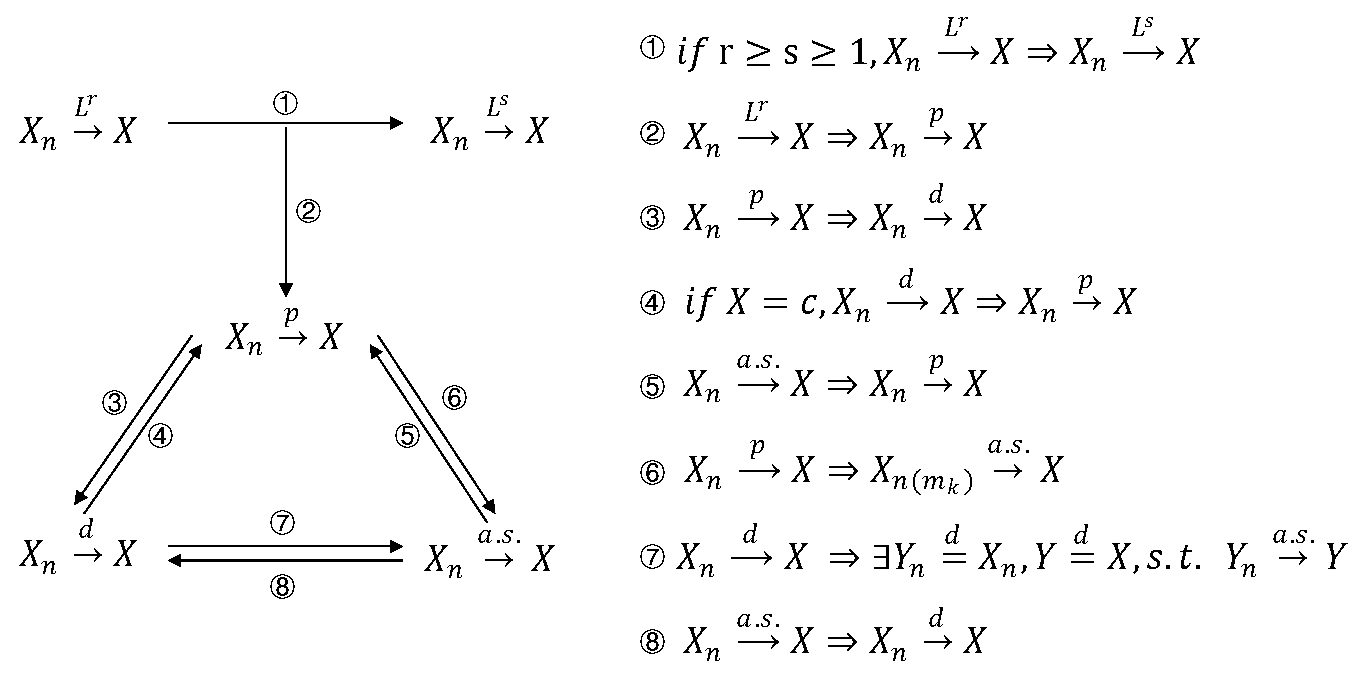
\includegraphics[width=0.9\textwidth]{./probability-theory/figures/relation-of-convergences.eps}
    \caption{Relations of Convergence of Random Variables}
\end{figure}

\section{Asymptotic Notation for Random Variables}

\begin{definition}
    A sequence $\{A_n\}$ of real-valued random variables is of smaller order in probability than a sequence $\{B_n\}$, if
    \begin{equation}
        \frac{A_n}{B_n}\stackrel{p}{\rightarrow}0.
    \end{equation}
    Smaller order in probability is denoted by
    \begin{equation}
        A_n=o_p(B_n).
    \end{equation}
    Particularly,
    \begin{equation}
        A_n=o_p(1)\iff A_n\stackrel{p}{\rightarrow}0.
    \end{equation}
\end{definition}

\begin{definition}
    A sequence $\{A_n\}$ of real-valued random variables is of smaller order than or equal to a sequence $\{B_n\}$ in probability, if
    \begin{equation}
        \forall\varepsilon>0\;\exists M_\varepsilon,\quad\lim_{n\rightarrow\infty} P\left(|A_n|\leq M_\varepsilon|B_n|\right)\geq 1-\varepsilon.
    \end{equation}
    Smaller order than or equal to in probability is denoted by
    \begin{equation}
        A_n=O_p(B_n).
    \end{equation}
\end{definition}

\begin{definition}
    A sequence $\{A_n\}$ of real-valued random variables is of the same order as a sequence $\{B_n\}$ in probability, if
    \begin{equation}
        \forall\varepsilon>0\;\exists m_{\varepsilon}<M_{\varepsilon},\quad\lim_{n\rightarrow\infty} P\left(m_{\varepsilon}<\frac{|A_{n}|}{|B_{n}|}<M_{\varepsilon}\right)\geq 1-\varepsilon.
    \end{equation}
    Same order in probability is denoted by
    \begin{equation}
        A_{n}\asymp_{p}B_{n}.
    \end{equation}
\end{definition}
\chapter{Law of Large Numbers}

\begin{introduction}
    \item Weak Law of Large Numbers
    \item Strong Law of Large Numbers
    \item Uniform Law of Large Numbers
\end{introduction}

\section{Weak Law of Large Numbers}

\begin{lemma}{}{}
    If $p>0$ and $E\left|Z_{n}\right|^{p}\rightarrow 0$, then
    \begin{equation}
        Z_{n}\stackrel{d}{\rightarrow}0.
    \end{equation}
\end{lemma}

\begin{proof}
    
\end{proof}

\begin{theorem}{Weak Law of Large Numbers with Finite Variances}{}
    Let $X_1,X_2,\ldots$ be i.i.d. random variables with $EX_i=\mu$ and $\text{Var}(X_i)\leq C<\infty$. Suppose $S_n=X_1+X_2+\ldots+X_n$, then
    \begin{equation}
        S_n/n\stackrel{L^2}{\rightarrow}\mu,\quad S_n/n\stackrel{p}{\rightarrow}\mu.
    \end{equation}
\end{theorem}

\begin{proof}
    
\end{proof}

\begin{theorem}{Weak Law of Large Numbers without i.i.d.}{}
    Let $X_1,X_2,\ldots$ be random variables, Suppose $S_n=X_1+X_2+\ldots+X_n$, $\mu_n=ES_n$, $\sigma_n^2=\text{Var}(S_n)$, if $\sigma_n^2/b_n^2\rightarrow 0$, then
    \begin{equation}
        \frac{S_n-\mu_n}{b_n}\stackrel{p}{\rightarrow}0.
    \end{equation}
\end{theorem}

\begin{proof}
    
\end{proof}

\begin{theorem}{Weak Law of Large Numbers for Triangular Arrays}{}
    For each $n$, let $X_{n,m},1\leq m\leq n$, be independent random variables. Suppose $b_n>0$ with $b_n\rightarrow\infty$, $\bar{X}_{n,m}=X_{n,m}I_{\left(X_{n,m}\leq b_n\right)}$, if
    \begin{enumerate}
        \item $\sum_{m=1}^{n}P\left(\left|X_{n,m}\right|>b_{n}\right)\rightarrow 0$, and
        \item $b_{n}^{-2}\sum_{m=1}^{n}E\bar{X}_{n,m}^{2}\rightarrow 0$.
    \end{enumerate}
    Suppose $S_{n}=X_{n, 1}+\cdots+X_{n,n}$ and $a_{n}=\sum_{m=1}^{n}E\bar{X}_{n,m}$, thenxxs
    \begin{equation}
        \frac{S_n-a_n}{b_n}\stackrel{p}{\rightarrow}0.
    \end{equation}
\end{theorem}

\begin{proof}
    
\end{proof}

\begin{theorem}{Weak Law of Large Numbers by Feller}{}
    Let $X_1,X_2,\ldots$ be i.i.d. random variables with
    \begin{equation}
        \lim_{x\rightarrow 0}xP(|X_i|>x)=0.
    \end{equation}
    Suppose $S_n=X_1+X_2+\ldots+X_n$, $\mu_n=E\left(X_1I_{(|X_1|<n)}\right)$, then
    \begin{equation}
        S_n/n-\mu_n\stackrel{p}{\rightarrow}0.
    \end{equation}
\end{theorem}

\begin{proof}
    
\end{proof}

\begin{theorem}{Weak Law of Large Numbers}{WLLN}
    Let $X_1,X_2,\ldots$ be i.i.d. random variables with $E|X_i|<\infty$. Suppose $S_n=X_1+X_2+\ldots+X_n$, $\mu=EX_i$, then
    \begin{equation}
        S_n/n\stackrel{p}{\rightarrow}\mu.
    \end{equation}
\end{theorem}

\begin{proof}
    
\end{proof}

\begin{note}
    $E|X_i|=\infty$
\end{note}

\section{Strong Law of Large Numbers}

\subsection{Borel-Cantelli Lemmas}

\begin{lemma}{Borel-Cantelli Lemma}{borel-cantelli-lemma}
    If $\sum_{n=1}^{\infty}P\left(A_{n}\right)<\infty$, then
    \begin{equation}
        P\left(A_{n}\text{ i.o. }\right)=0.
    \end{equation}
\end{lemma}

\begin{lemma}{The Second Borel-Cantelli Lemma}{}
    If $\{A_n\}$ are independent with $\sum_{n=1}^{\infty}P\left(A_{n}\right)=\infty$, then,
    \begin{equation}
        P\left(A_{n}\text{ i.o. }\right)=1.
    \end{equation}
\end{lemma}

\begin{corollary}{}{}
    Suppose $\{A_{n}\}$ are independent with $P\left(A_{n}\right)<1,\forall n$. If $P\left(\cup_{n=1}^{\infty}A_{n}\right)=1$ then
    \begin{equation}
        \sum_{n=1}^{\infty}P\left(A_{n}\right)=\infty,
    \end{equation}
    and hence $P\left(A_{n}\text{ i.o. }\right)=1$
\end{corollary}

\begin{proof}

\end{proof}

\subsection{Strong Law of Large Numbers}

\begin{theorem}{Strong Law of Large Numbers}{SLLN}
    Let $X_1,X_2,\ldots$ be i.i.d. random variables with $E|X_i|<\infty$. Suppose $S_n=X_1+X_2+\ldots+X_n$, $\mu=EX_i$, then
    \begin{equation}
        S_n/n\stackrel{a.s.}{\rightarrow}\mu.
    \end{equation}
\end{theorem}

\section{Uniform Law of Large Numbers}

\begin{theorem}{Uniform Law of Large Numbers}{ULLN}
    Suppose
    \begin{enumerate}
        \item $\Theta$ is compact.
        \item $g\left(X_{i},\theta\right)$ is continuous at each $\theta\in\Theta$ almost sure.
        \item $g\left(X_{i},\theta\right)$ is dominated by a function $G\left(X_{i}\right)$, i.e. $\left|g\left(X_{i},\theta\right)\right|\leq G\left(X_{i}\right)$.
        \item $EG\left(X_{i}\right)<\infty$.
    \end{enumerate}
    Then
    \begin{equation}
        \sup_{\theta\in\Theta}\left|n^{-1}\sum_{i=1}^{n}g\left(X_{i},\theta\right)-Eg\left(X_{i},\theta\right)\right|\stackrel{p}{\rightarrow}0.
    \end{equation}
\end{theorem}

\begin{proof}
    
\end{proof}

\chapter{Central Limit Theorems}

% \begin{introduction}
%     \item Classic Central Limit Theorem
%     \item Central Limit Theorem for independent non-identical Random Variables
%     \item Central Limit Theorem for dependent Random Variables
% \end{introduction}

\section{Classic Central Limit Theorem}

\subsection{The De Moivre-Laplace Theorem}

\begin{lemma}[Stirling's Formula] \label{lem:stirling}
    \begin{equation}
        n ! \sim \sqrt{2 \pi} n^{n+\frac{1}{2}} e^{-n} \text{ as } n \rightarrow \infty.
    \end{equation}
\end{lemma}

\begin{proof}

\end{proof}

\begin{lemma} \label{lem:exp}
    If $c_j\rightarrow 0$, $a_j\rightarrow\infty$ and $a_jc_j\rightarrow\lambda$, then
    \begin{equation}
        \left(1+c_j\right)^{a_j}\rightarrow e^\lambda.
    \end{equation}
\end{lemma}

\begin{proof}

\end{proof}

\begin{theorem}[The De Moivre-Laplace Theorem] \label{thm:de-moivre-laplace}
    Let $X_{1}, X_{2}, \ldots$ be i.i.d. with $P\left(X_{1}=1\right)=P\left(X_{1}=-1\right)=1 / 2$ and let $S_{n}=X_{1}+\cdots+X_{n}$. If $a<b$, then as $m \rightarrow \infty$
    \begin{equation}
        P\left(a \leq S_{m} / \sqrt{m} \leq b\right) \rightarrow \int_{a}^{b}(2 \pi)^{-1 / 2} e^{-x^{2} / 2} \mathrm{d} x.
    \end{equation}
\end{theorem}

\begin{proof}
    If $n$ and $k$ and integers
    \begin{equation*}
        P\left(S_{2 n}=2 k\right)=\left(\begin{array}{c}
                2 n \\
                n+k
            \end{array}\right) 2^{-2 n}
    \end{equation*}
    By lemma \ref{lem:stirling}, we have
    \begin{equation*}
        \begin{aligned}
            \left(\begin{array}{c}
                    2 n \\
                    n+k
                \end{array}\right) & =\frac{(2 n) !}{(n+k) !(n-k) !}                                                                                             \\
                                                   & \sim \frac{(2 n)^{2 n}}{(n+k)^{n+k}(n-k)^{n-k}} \cdot \frac{(2 \pi(2 n))^{1 / 2}}{(2 \pi(n+k))^{1 / 2}(2 \pi(n-k))^{1 / 2}}
        \end{aligned}
    \end{equation*}
    Hence,
    \begin{equation*}
        \begin{aligned}
            P\left(S_{2 n}=2 k\right) & =
            \left(\begin{array}{c}
                    2 n \\
                    n+k
                \end{array}\right) 2^{-2 n}                                                                                               \\
                                      & \sim\left(1+\frac{k}{n}\right)^{-n-k} \cdot\left(1-\frac{k}{n}\right)^{-n+k}                                      \\
                                      & \cdot(\pi n)^{-1 / 2} \cdot\left(1+\frac{k}{n}\right)^{-1 / 2} \cdot\left(1-\frac{k}{n}\right)^{-1 / 2}           \\
                                      & =\left(1-\frac{k^{2}}{n^{2}}\right)^{-n} \cdot\left(1+\frac{k}{n}\right)^{-k} \cdot\left(1-\frac{k}{n}\right)^{k} \\
                                      & \cdot(\pi n)^{-1 / 2} \cdot\left(1+\frac{k}{n}\right)^{-1 / 2} \cdot\left(1-\frac{k}{n}\right)^{-1 / 2}           \\
        \end{aligned}
    \end{equation*}
    Let $2k=x\sqrt{2n}$, i.e., $k=x\sqrt{\frac{n}{2}}$. By lemma \ref{lem:exp}, we have
    \begin{equation*}
        \begin{aligned}
            \left(1-\frac{k^{2}}{n^{2}}\right)^{-n} & =\left(1-x^{2} / 2 n\right)^{-n} \rightarrow e^{x^{2} / 2}       \\
            \left(1+\frac{k}{n}\right)^{-k}         & =(1+x / \sqrt{2 n})^{-x \sqrt{n / 2}} \rightarrow e^{-x^{2} / 2} \\
            \left(1-\frac{k}{n}\right)^{k}          & =(1-x / \sqrt{2 n})^{x \sqrt{n / 2}} \rightarrow e^{-x^{2} / 2}
        \end{aligned}
    \end{equation*}
    For this choice of $k$, $k/n \rightarrow 0$, so
    \begin{equation*}
        \left(1+\frac{k}{n}\right)^{-1 / 2} \cdot\left(1-\frac{k}{n}\right)^{-1 / 2} \rightarrow 1.
    \end{equation*}
    Putting things together, we have
    \begin{equation*}
        P\left(S_{2 n}=2 k\right) \sim (\pi n)^{-1 / 2} e^{-x^{2} / 2}, \text{ as } \frac{2k}{\sqrt{2n}} \rightarrow x.
    \end{equation*}
    Therefore,
    \begin{equation*}
        P\left( a\sqrt{2n} \leq S_{2 n} \leq b\sqrt{2 n} \right) = \sum_{m \in \left[a\sqrt{2 n},b\sqrt{2 n}\right] \cap 2\mathbb{Z}} P\left(S_{2 n}=m\right)
    \end{equation*}
    Let $m=x\sqrt{2 n}$, we have that this is
    \begin{equation*}
        \approx \sum_{x \in \left[a,b\right] \cap \left(2\mathbb{Z} / \sqrt{2 n}\right)}(2 \pi)^{-1 / 2} e^{-x^{2} / 2}\cdot(2/n)^{1/2}
    \end{equation*}
    where $2\mathbb{Z} / \sqrt{2 n} = \left\{2z/\sqrt{2n} : z\in\mathbb{Z}\right\}$. As $n\rightarrow\infty$, the sum just shown is
    \begin{equation*}
        \approx \int_{a}^{b}(2 \pi)^{-1 / 2} e^{-x^{2} / 2} \mathrm{d} x.
    \end{equation*}
    To remove the restriction to even integers, observe $S_{2 n +1}=S_{2 n} \pm 1$.\\
    Let $m=2n$, as $m\rightarrow\infty$,
    \begin{equation*}
        P\left(a \leq S_{m} / \sqrt{m} \leq b\right) \rightarrow \int_{a}^{b}(2 \pi)^{-1 / 2} e^{-x^{2} / 2} \mathrm{d} x.
    \end{equation*}
\end{proof}

\subsection{Classic Central Limit Theorem}

\begin{theorem}[Classic Central Limit Theorem (i.i.d.)]
    Let $X_1,X_2,\ldots$ be i.i.d. with $EX_i=\mu$, $\text{Var}(X_i)=\sigma^2<\infty$. Let $S_n=X_1+X_2+\ldots+X_n$, then
    \begin{equation}
        \frac{S_n-n\mu}{\sigma n^{\frac{1}{2}}} \stackrel{d}{\rightarrow} \chi,
    \end{equation}
    where $\chi$ has the standard normal distribution.
\end{theorem}

\begin{proof}

\end{proof}

\begin{theorem}[The Linderberg-Feller Central Limit Theorem]
    For each $n$, let $X_{n,m},1\leq m\leq n$, be independent random variables with $EX_{n,m}=0$. If
    \begin{enumerate}
        \item $\sum_{m=1}^{n}EX_{n,m}^{2} \rightarrow \sigma^{2}>0$.
        \item $\forall\epsilon>0,\lim_{n\rightarrow\infty}\sum_{m=1}^{n}E\left(\left|X_{n,m}\right|^{2};\left|X_{n,m}\right|>\epsilon\right)=0$
    \end{enumerate}
    Then $S_{n}=X_{n,1}+\cdots+X_{n,n}\stackrel{d}{\rightarrow}\sigma\chi$ as $n\rightarrow\infty$.
\end{theorem}

\subsection{Berry-Esseen Theorem}

\begin{theorem}[Berry-Esseen Theorem]
    Let $X_{1},X_{2},\ldots,X_{n}$ be i.i.d. with distribution $F$ , which has a mean $\mu$ and a finite third moment $\sigma^{3}$, then there exists a constant $C$ (independent of $F$),
    \begin{equation}
        \left|G_{n}(x)-\Phi(x)\right|\leq\frac{C}{\sqrt{n}}\frac{E\left|X_{1}-\mu\right|^{3}}{\sigma^{3}},\quad\forall x.
    \end{equation}
\end{theorem}

\begin{corollary}
    Under the assumptions of Theorem 51 ,
    $$
        G_{n}(x) \rightarrow \Phi(x) \text { as } n \rightarrow \infty
    $$
    for any sequence $F_{n}$ with mean $\xi_{n}$ and variance $\sigma_{n}^{2}$ for which
    $$
        \frac{E_{n}\left|X_{1}-\xi_{n}\right|^{3}}{\sigma_{n}^{3}}=o(\sqrt{n})
    $$
    and thus in particular if $(72)$ is bounded. Here $E_{n}$ denotes the expectation under $F_{n}$.
\end{corollary}

\section{Central Limit Theorem for independent non-identical Random Variables}

\begin{theorem}[The Liapounov Central Limit Theorem]

\end{theorem}

\section{Central Limit Theorem for Dependent Random Variables}

\chapter{Exercises for Probability Theory and Examples}

\section{Measure Theory}

\begin{exercise}
    \begin{enumerate}
        \item Show that if $\mathcal{F}_{1}\subset \mathcal{F}_{2}\subset\ldots$ are $\sigma$ -algebras, then $\cup_{i}\mathcal{F}_{i}$ is an algebra.
        \item Give an example to show that $\cup_{i}\mathcal{F}_{i}$ need not be a $\sigma$ -algebra.
    \end{enumerate}
\end{exercise}

\begin{proof}
    \begin{enumerate}
        \item
              \textbf{Complement}: Suppose $A\in\cup_{i}\mathcal{F}_{i}$, since $\mathcal{F}_{1}\subset \mathcal{F}_{2}\subset\ldots$, assume $A\in\mathcal{F}_{i}$. And each $\mathcal{F}_{i}$ is $\sigma$-algebra,
              \begin{equation*}
                  A^c\in\mathcal{F}_{i}\subset\cup_{i}\mathcal{F}_{i}.
              \end{equation*}
              \textbf{Finite Union}: Suppose $A_1,A_2\in\cup_{i}\mathcal{F}_{i}$, since $\mathcal{F}_{1}\subset \mathcal{F}_{2}\subset\ldots$, assume $A_1\in\mathcal{F}_{i},A_2\in\mathcal{F}_{j}$, such that,
              \begin{equation*}
                  A_1,A_2\in\mathcal{F}_{\max(i,j)}.
              \end{equation*}
              Since each $\mathcal{F}_{i}$ is $\sigma$-algebra,
              \begin{equation*}
                  A_1\cup A_2\in\mathcal{F}_{i}\subset\cup_{i}\mathcal{F}_{i}.
              \end{equation*}
        \item
              Let $\mathcal{F}_{i}$ be a Borel Set of $[1,2-\frac{1}{i}]$. Suppose $A_i=[1,2-\frac{1}{i}]\in\mathcal{F}_{i}$,
              \begin{equation*}
                  \cup_{i}A_{i}=[1,2)\notin\cup_{i}\mathcal{F}_{i}.
              \end{equation*}
    \end{enumerate}
\end{proof}

\section{Laws of Large Numbers}

\section{Central Limit Theorems}

\begin{exercise}
    Let $g\geq 0$ be continuous. If $X_{n}\stackrel{d}{\rightarrow}X_{\infty},$ then
    \begin{equation*}
        \liminf_{n\rightarrow\infty}Eg\left(X_{n}\right)\geq Eg\left(X_{\infty}\right).
    \end{equation*}
    \label{ex:fatou-lemma-distribution}
\end{exercise}

\begin{proof}
    Let $Y_n\stackrel{d}{=}X_n,1\leq n\leq\infty$ with $Y_n\stackrel{a.s.}{\rightarrow}Y_\infty$ (Lemma \ref{lem:distribution-to-probability}).
    Since $g\geq 0$ be continuous, $g(Y_n)\stackrel{a.s.}{\rightarrow}g(Y_\infty)$ and $g(Y_n)\geq 0$ (Theorem \ref{thm:continuous-mapping-theorem}), and the Fatou's Lemma (\ref{thm:fatou-lemma}) implies,
    \begin{equation*}
        \begin{aligned}
            \liminf_{n\rightarrow\infty}Eg(X_n)= & \liminf_{n\rightarrow\infty}Eg(Y_n)\geq E\left(\liminf_{n\rightarrow\infty}g(Y_n)\right) \\
            =                                    & Eg(Y_\infty)=Eg(X_\infty).
        \end{aligned}
    \end{equation*}
\end{proof}

\begin{exercise}
    Suppose $g,h$ are continuous with $g(x)>0$, and $|h(x)|/g(x)\rightarrow 0$ as $|x|\rightarrow\infty$. If $F_{n}\stackrel{d}{\rightarrow}F$ and $\int g(x)\mathrm{d}F_{n}(x)\leq C<\infty,$ then
    \begin{equation*}
        \int h(x)\mathrm{d}F_{n}(x) \rightarrow \int h(x)\mathrm{d}F(x).
    \end{equation*}
\end{exercise}

\begin{proof}
    \begin{equation*}
        \begin{aligned}
            \left|\int h(x)\mathrm{d}F_{n}(x)-\int h(x)\mathrm{d}F(x)\right| = & \left|{\int_{x\in[-M,M]}h(x)\mathrm{d}F_{n}(x)+\int_{x\notin[-M,M]}h(x)\mathrm{d}F_{n}(x)}\right. \\
                                                                               & \left.{-\int_{x\in[-M,M]}h(x)\mathrm{d}F(x)-\int_{x\notin[-M,M]}h(x)\mathrm{d}F(x)}\right|        \\
            \leq                                                               & \left|\int_{x\in[-M,M]}h(x)\mathrm{d}F_{n}(x)-\int_{x\in[-M,M]}h(x)\mathrm{d}F(x)\right|          \\
                                                                               & + \left|\int_{x\notin[-M,M]}h(x)\mathrm{d}F_{n}(x)-\int_{x\notin[-M,M]}h(x)\mathrm{d}F(x)\right|
        \end{aligned}.
    \end{equation*}

    Let $X_n,1\leq n<\infty$, with distribution $F_n$, so that $X_n\stackrel{a.s.}{\rightarrow}X$ (Lemma \ref{lem:distribution-to-probability}).
    \begin{equation*}
        \left|\int_{x\in[-M,M]}h(x)\mathrm{d}F_{n}(x)-\int_{x\in[-M,M]}h(x)\mathrm{d}F(x)\right| = \left|E\left(h(X_n)-h(X)\right)I_{x\in[-M,M]}\right|.
    \end{equation*}

    By Continuity Mapping Theorem (\ref{thm:continuous-mapping-theorem}), $\lim_{n\rightarrow\infty}\left|E\left(h(X_n)-h(X)\right)I_{x\in[-M,M]}\right| = 0$.

    Since
    \begin{equation*}
        h(x)I_{x\notin[-M,M]}\leq g(x)\sup_{x\notin[-M,M]}\frac{h(x)}{g(x)},
    \end{equation*}
    and by Exercise \ref{ex:fatou-lemma-distribution}
    \begin{equation*}
        Eg(X) \leq \liminf_{n\rightarrow\infty}Eg(X_n)=\liminf_{n\rightarrow\infty}\int g(x)\mathrm{d}F_{n}(x)\leq C<\infty,
    \end{equation*}
    \begin{equation*}
        \begin{aligned}
            \left|\int_{x\notin[-M,M]}h(x)\mathrm{d}F_{n}(x)-\int_{x\notin[-M,M]}h(x)\mathrm{d}F(x)\right| = \left|E\left(h(X_n)-h(X)\right)I_{x\notin[-M,M]}\right| \\
            \leq 2E\max(h(Xn),h(X))I_{x\notin[-M,M]}\leq 2C\sup_{x\notin[-M,M]}\frac{h(x)}{g(x)}.                                                                    \\
        \end{aligned}
    \end{equation*}

    Hence, let $M\rightarrow\infty$,
    \begin{equation*}
        \lim_{n\rightarrow\infty}\left|\int h(x)\mathrm{d}F_{n}(x)-\int h(x)\mathrm{d}F(x)\right| \leq 2C\sup_{x\notin[-M,M]}\frac{h(x)}{g(x)}\rightarrow 0,
    \end{equation*}
    which means,
    \begin{equation*}
        \int h(x)\mathrm{d}F_{n}(x) \rightarrow \int h(x)\mathrm{d}F(x).
    \end{equation*}
\end{proof}

\begin{exercise}
    Let $X_{1},X_{2},\ldots$ be i.i.d. with $EX_{i}=0$ and $EX_{i}^{2}=\sigma^{2}\in(0,\infty)$. Then
    \begin{equation*}
        \sum_{m=1}^{n}X_{m}/\left(\sum_{m=1}^{n}X_{m}^{2}\right)^{1/2}\stackrel{d}{\rightarrow}\chi.
    \end{equation*}
\end{exercise}

\begin{exercise}
    Show that if $\left|X_{i}\right|\leq M$ and $\sum_{n}\text{Var}\left(X_{n}\right)=\infty$, then
    \begin{equation*}
        \left(S_{n}-E S_{n}\right)/\sqrt{\text{Var}\left(S_{n}\right)}\stackrel{d}{\rightarrow}\chi.
    \end{equation*}
\end{exercise}

\begin{exercise}
    Suppose $EX_{i}=0,EX_{i}^{2}=1$ and $E\left|X_{i}\right|^{2+\delta}\leq C$ for some $0<\delta,C<\infty$. Show that
    \begin{equation*}
        S_{n}/\sqrt{n}\stackrel{d}{\rightarrow}\chi.
    \end{equation*}
\end{exercise}

\part{Stochastic Process}
\chapter{Martingales}

\section{Conditional Expectation}

\begin{definition}[Conditional Expectation]

\end{definition}

\begin{example}
    \begin{enumerate}
        \item
    \end{enumerate}
\end{example}

\begin{property}
    
\end{property}

\section{Martingales}

Let $\mathcal{F}_{n}$ be a filtration, i.e., an increasing sequence of $\sigma$-fields.
\begin{definition}[Martingale]
    A sequence $\left\{X_{n}\right\}$ of real-valued random variables  is said to be a martingale with respect to $\mathcal{F}_{n}$, if
    \begin{enumerate}
        \item $X_{n}$ is integrable, i.e., $E\left|X_{n}\right|<\infty$
        \item $X_{n}$ is adapted to $\mathcal{F}_{n}$, i.e., $\forall n,X_{n}\in \mathcal{F}_{n}$
        \item $X_{n}$ satisfies the martingale condition, i.e.,
              \begin{equation}
                  E\left(X_{n+1}\mid\mathcal{F}_{n}\right)=X_{n},\quad\forall n
              \end{equation}
    \end{enumerate}
\end{definition}

\begin{note}
    If in the last definition $=$ is replaced by $\leq$ or $\geq$, then $X$ is said to be a supermartingale or submartingale, respectively.
\end{note}

\begin{example}[ Linear Martingale]
    
\end{example}

\begin{example}[ Quadratic Martingale]
    
\end{example}

\begin{example}[ Random Walk]
    Suppose $X_{n}=X_{0}+\xi_{1}+\cdots+\xi_{n}$, where $X_{0}$ is constant, $\xi_{m}$ are independent and have $E\xi_{m}=0,\sigma_{m}^{2}=E\xi_{m}^{2}<\infty$. Let $\mathcal{F}_{n}=\sigma\left(\xi_{1},\ldots,\xi_{n}\right)$ for $n\geq 1$ and take $\mathcal{F}_{0}=\{\emptyset, \Omega\}$. Show $X_{n}$ is a martingale, and $X_{n}^{2}$ is a submartingale.
\end{example}

\begin{proof}
    It is obvious that,
    \begin{equation*}
        E\left|X_{n}\right|<\infty,\quad X_{n}\in\mathcal{F}_{n}
    \end{equation*}
    Since $\xi_{n+1}$ is independent of $\mathcal{F}_{n}$, so using the linearity of conditional expectation, (4.1.1), and Example 4.1.4,
    \begin{equation*}
        E\left(X_{n+1}\mid\mathcal{F}_{n}\right)=E\left(X_{n}\mid\mathcal{F}_{n}\right)+E\left(\xi_{n+1}\mid\mathcal{F}_{n}\right)=X_{n}+E\xi_{n+1}=X_{n}
    \end{equation*}
    So $X_{n}$ is a martingale, and Theorem 4.2.6 implies $X_{n}^{2}$ is a submartingale.
\end{proof}

\begin{note}
    If we let $\lambda=x^{2}$ and apply Theorem 4.4.2 to $X_{n}^{2}$, we get Kolmogorov's maximal inequality, Theorem 2.5.5:
    \begin{equation}
        P\left(\max_{1\leq m\leq n}\left|X_{m}\right|\geq x\right)\leq x^{-2}\operatorname{var}\left(X_{n}\right)
    \end{equation}
\end{note}

\section{Doob's Inequality}

\begin{theorem}[Doob's Decomposition]

\end{theorem}

\begin{theorem}[Doob's Inequality]

\end{theorem}

\begin{theorem}[$L^{p}$ Maximum Inequality]

\end{theorem}

\section{Uniform Integrability}

\section{Optional Stopping Theorems}

\chapter{Exercises for Probability Theory and Examples}

\section{Martingales}

\section{Markov Chains}

\section{Ergodic Theorems}

\section{Brownian Motion}

\section{Applications to Random Walk}

\section{Multidimensional Brownian Motion}
\chapter{Markov Chains}

\section{Markov Chain}

\begin{definition}[Markov Chain, Simple]
    A sequence $\left\{X_{n}\right\}$ of real-valued random variables  is said to be a Markov chain, if for any states $i_{0},\ldots i_{n-1},i$, and $j$
    \begin{equation}
        P\left(X_{n+1}=j\mid X_{n}=i,X_{n-1}=i_{n-1},\ldots X_{0}=i_{0}\right)=P\left(X_{n+1}=j\mid X_{n}=i\right)
    \end{equation}
    and the transition probability is
    \begin{equation}
        p(i,j)=P\left(X_{n+1}=j\mid X_{n}=i\right)
    \end{equation}
\end{definition}

\begin{example}[ Random Walk]
    Suppose $X_{n}=X_{0}+\xi_{1}+\cdots+\xi_{n}$, where $X_{0}$ is constant, $\xi_{m}\in\mathbb{Z}^{d}$ are independent with distribution $\mu$. Show $X_{n}$ is a Markov chain with transition probability,
    \begin{equation*}
        p\left(i,j\right)=\mu\left(\left\{j-i\right\}\right)
    \end{equation*}
\end{example}

\begin{proof}
    Since $\xi_{m}$ are independent with distribution $\mu$,
    \begin{equation*}
        \begin{aligned}
              & P\left(X_{n+1}=j\mid X_{n}=i,X_{n-1}=i_{n-1},\ldots X_{0}=i_{0}\right)                                     \\
            = & P\left(X_{n}+\xi_{n+1}=j\mid X_{n}=i\right)=P\left(\xi_{n+1}=j-i\right)=\mu\left(\left\{j-i\right\}\right)
        \end{aligned}
    \end{equation*}
\end{proof}

\begin{definition}[Branching Processes]
    Let $\xi_{i}^{n},i,n\geq 1$, be i.i.d. nonnegative integer-valued random variables. Define a sequence $Z_{n},n\geq 0$ by $Z_{0}=1$ and
    \begin{equation}
        Z_{n+1}=\left\{\begin{array}{ll}
            \xi_{1}^{n+1}+\cdots+\xi_{Z_{n}}^{n+1} & Z_{n}>0 \\
            0                                      & Z_{n}=0
        \end{array}\right.
    \end{equation}
    $Z_{n}$ is called a Branching process.
\end{definition}

\begin{note}
    The idea behind the definitions is that $Z_{n}$ is the number of individuals in the $n$-th generation, and each member of the $n$-th generation gives birth independently to an identically distributed number of children.
\end{note}

\begin{example}[ Branching Processes]
    Show branching process is a Markov chain with transition probability,
    \begin{equation*}
        p(i,j)=P\left(\sum_{k=1}^{i}\xi_{k}=j\right)
    \end{equation*}
\end{example}

\begin{proof}
    Since $\xi_{k}^{n}$ are independent with identically distribution,
    \begin{equation*}
        \begin{aligned}
              & P\left(Z_{n+1}=j\mid Z_{n}=i,Z_{n-1}=i_{n-1},\ldots Z_{0}=i_{0}\right)                            \\
            = & P\left(\sum_{k=1}^{Z_{n}}\xi_{k}^{n+1}=j\mid Z_{n}=i\right)=P\left(\sum_{k=1}^{i}\xi_{k}=j\right)
        \end{aligned}
    \end{equation*}
\end{proof}

Suppose $(S, \mathcal{S})$ be a measurable space, which will be the state space for our Markov chain.

\begin{definition}[Transition Probability]
    A function $p:S\times\mathcal{S}\rightarrow\mathbf{R}$ is said to be a transition probability, if
    \begin{enumerate}
        \item For each $x\in S$, $A\rightarrow p(x,A)$ is a probability measure on $(S,\mathcal{S})$
        \item For each $A\in\mathcal{S}$, $x\rightarrow p(x,A)$ is a measurable function
    \end{enumerate}
\end{definition}
\begin{definition}[Markov Chain]
    A sequence $\left\{X_{n}\right\}$ of real-valued random variables with transition probability $p$ is said to be a Markov chain with respect to $\mathcal{F}_{n}$, if
    \begin{equation}
        P\left(X_{n+1}\in B\mid\mathcal{F}_{n}\right)=p\left(X_{n},B\right)
    \end{equation}
\end{definition}

\begin{remark}
    Given a transition probability $p$ and an initial distribution $\mu$ on $(S,\mathcal{S})$, the consistent set of finite dimensional distributions is
    \begin{equation}
        P\left(X_{j}\in B_{j},0\leq j\leq n\right)=\int_{B_{0}}\mu\left(\,\mathrm{d}x_{0}\right)\int_{B_{1}}p\left(x_{0},\,\mathrm{d}x_{1}\right)\cdots\int_{B_{n}}p\left(x_{n-1},\,\mathrm{d}x_{n}\right)
        F    \end{equation}
\end{remark}

\section{Markov Properties}

\begin{theorem}[Markov Property]

\end{theorem}

\begin{corollary}[Chapman-Kolmogorov Equation]

\end{corollary}

\begin{theorem}[Strong Markov Property]

\end{theorem}

\section{Recurrence and Transience}

Let $T_{y}^{0}=0$, and for $k\geq 1$, and
\begin{equation}
    T_{y}^{k}=\inf\left\{n>T_{y}^{k-1}:X_{n}=y\right\}
\end{equation}
then $T_{y}^{k}$ is the time of the $k$-th return to $y$, where $T_{y}^{1}>0$, so any visit at time 0 does not count.

Let
\begin{equation}
    \rho_{x y}=P_{x}\left(T_{y}<\infty\right)
\end{equation}
and we have
\begin{equation}
    P_{x}\left(T_{y}^{k}<\infty\right)=\rho_{xy}\rho_{yy}^{k-1}
\end{equation}

\begin{proof}

\end{proof}

Let
\begin{equation}
    N(y)=\sum_{n=1}^{\infty}1_{\left(X_{n}=y\right)}
\end{equation}
be the number of visits to $y$ at positive times.

\begin{definition}[Recurrent]
    A state $y$ is said to be recurrent if $\rho_{yy}=1$.
\end{definition}

\begin{property}
    The recurrent state $y$ has the following properties
    \begin{enumerate}
        \item $y$ is recurrent if and only if
              \begin{equation*}
                  E_{y}N(y)=\infty.
              \end{equation*}
        \item If $x$ is recurrent and $\rho_{xy}>0$, then $y$ is recurrent and $\rho_{yx}=1$.
    \end{enumerate}
\end{property}

\begin{definition}
    A state $y$ is said to be transient if $\rho_{yy}<1$.
\end{definition}

\begin{property}
    The transient state $y$ has the following properties
    \begin{enumerate}
        \item If $y$ is transient, then
              \begin{equation*}
                  E_{x}N(y)<\infty,\quad\forall x.
              \end{equation*}
    \end{enumerate}
\end{property}

\begin{proof}
    \begin{equation*}
        \begin{aligned}
            E_{x}N(y) & =\sum_{k=1}^{\infty}P_{x}(N(y)\geq k)=\sum_{k=1}^{\infty}P_{x}\left(T_{y}^{k}<\infty\right) \\
                      & =\sum_{k=1}^{\infty}\rho_{xy}\rho_{yy}^{k-1}=\frac{\rho_{xy}}{1-\rho_{yy}}<\infty
        \end{aligned}
    \end{equation*}
\end{proof}

\begin{definition}[Closed State Set]
    A set $C$ of states is said to be closed, if
    \begin{equation}
        x\in C,\rho_{xy}>0\Rightarrow y\in C.
    \end{equation}
\end{definition}

\begin{definition}[Irreducible State Set]
    A set $D$ of states is said to be irreducible, if
    \begin{equation}
        x,y\in D\Rightarrow\rho_{xy}>0.
    \end{equation}
\end{definition}

\begin{theorem}
    Let $C$ be a finite closed set, then
    \begin{enumerate}
        \item $C$ contains a recurrent state.
        \item If $C$ is irreducible, then all states in $C$ are recurrent.
    \end{enumerate}
\end{theorem}

\begin{theorem}
    Suppose $C_{x}=\left\{y:\rho_{x y}>0\right\}$, then $C_{x}$ is an irreducible closed set.
\end{theorem}

\begin{proof}
    If $y,z\in C_{x}$, then $\rho_{yz}\geq\rho_{yx}\rho_{xz}>0$. If $\rho_{yw}>0$, then $\rho_{xw}\geq\rho_{xy}\rho_{yw}>0$, so $w\in C_{x}$.
\end{proof}

\begin{example}[ A Seven-state Chain]
    Consider the transition probability,
    \begin{equation*}
        \begin{array}{cccccccc}
                       & \mathbf{1} & \mathbf{2} & \mathbf{3} & \mathbf{4} & \mathbf{5} & \mathbf{6} & \mathbf{7} \\
            \mathbf{1} & .3         & 0          & 0          & 0          & .7         & 0          & 0          \\
            \mathbf{2} & .1         & .2         & .3         & .4         & 0          & 0          & 0          \\
            \mathbf{3} & 0          & 0          & .5         & .5         & 0          & 0          & 0          \\
            \mathbf{4} & 0          & 0          & 0          & .5         & 0          & .5         & 0          \\
            \mathbf{5} & .6         & 0          & 0          & 0          & .4         & 0          & 0          \\
            \mathbf{6} & 0          & 0          & 0          & .1         & 0          & .1         & .8         \\
            \mathbf{7} & 0          & 0          & 0          & 1          & 0          & 0          & 0
        \end{array}
    \end{equation*}
    try to identify the states that are recurrent and those that are transient.
\end{example}

\begin{proof}
    $\{2,3\}$ are transition states, and $\{1,4,5,6,7\}$ are recurrent states.
\end{proof}

\begin{remark}
    Suppose $S$ is finite, for $x\in S$,
    \begin{enumerate}
        \item $x$ is transient, if
              \begin{equation*}
                  \exists y,\text{ s.t. }\quad\rho_{xy}>0,\rho_{yx}=0
              \end{equation*}
        \item $x$ is recurrent, if
              \begin{equation*}
                  \exists y,\text{ s.t. }\quad\rho_{xy}>0,\rho_{yx}>0
              \end{equation*}
    \end{enumerate}
\end{remark}

% Theorem 5.2.6 implies $P_{y}\left(T_{y}^{k}<\infty\right)=1$ for all $k$, so $P_{y}\left(X_{n}=y\text{ i.o. }\right)=1$.

\section{Stationary Measures}

\section{Asymptotic Behavior}

\section{Ergodic Theorems}

\begin{definition}[Stationary Sequence]

\end{definition}

\begin{theorem}[Ergodic Theorem]

\end{theorem}

\begin{example}

\end{example}

\part{Statistics Inference}
\chapter{Introduction}

\section{Populations and Samples}

\section{Statistics}

\subsection{Sufficient Statistics}

\begin{definition}{Sufficient Statistics}{}
    A statistic $T$ is said to be sufficient for $X$, or for the family $\mathcal{P}=\left\{P_{\theta}, \theta \in \Omega\right\}$ of possible distributions of $X$, or for $\theta$, if the conditional distribution of $X$ given $T=t$ is independent of $\theta$ for all $t$.
\end{definition}

\begin{theorem}{Fisher–Neyman Factorization Theorem}{}
    If the probability density function is $p_{\theta}(x)$, then $T$ is sufficient for $\theta$ if and only if nonnegative functions $g$ and $h$ can be found such that
    \begin{equation*}
        p_{\theta}(x)=h(x)g_{\theta}[T(x)].
    \end{equation*}
\end{theorem}

\begin{proof}
    
\end{proof}

\subsection{Completeness}

\section{Estimators}

\subsection{Definition of Estimators}

\begin{definition}{Estimator}{estimator}
    An estimator is a real-valued function defined over the sample space, that is
    \begin{equation}
        \delta:\textbf{X}\rightarrow\mathbb{R}.
    \end{equation}
    It is used to estimate an estimand, $g(\theta)$, a real-valued function of the parameter.
\end{definition}

\subsection{Properties of Estimators}

\subsubsection*{Unbiasedness}

\begin{definition}{Unbiasedness}{}
    An estimator $\delta(\textbf{X})$ of $g(\theta)$ is unbiased if
    \begin{equation}
        E_\theta\left[\delta(\textbf{X})\right]=g(\theta),\quad\forall\theta\in\Theta.
    \end{equation}
\end{definition}

\begin{note}
    \begin{itemize}
        \item Unbiased estimators of $g(\theta)$ may not exist.
        \item 
    \end{itemize}
\end{note}

\begin{example}[ Nonexistence of Unbiased Estimator ]
    
\end{example}

\subsubsection*{Consistency}

\begin{definition}{Consistency}{}
    
\end{definition}

\subsubsection*{Asymptotic Normality}

\begin{definition}{Asymptotic Normality}{}
    
\end{definition}

\subsubsection*{Efficiency}

\begin{definition}{Efficiency}{}
    
\end{definition}

\subsubsection*{Robustness}

\begin{definition}{Robustness}{}
    
\end{definition}

\chapter{Maximum Likelihood Estimator}

Suppose that $\textbf{X}_{n}=\left(X_{1},\ldots,X_{n}\right)$, where the $X_{i}$ are i.i.d. with common density $p\left(x;\theta_{0}\right)\in\mathcal{P}=\{p(x;\theta):\theta\in\Theta\}$.

We assume that

\begin{quotation}
    $\theta_{0}$ is identified in the sense that if $\theta\neq\theta_{0}$ and $\theta\in\Theta$, then $p(x;\theta)\neq p\left(x;\theta_{0}\right)$ with respect to the dominating measure $\mu$.
\end{quotation}

For fixed $\theta\in\Theta$, the joint density of $\textbf{X}_{n}$ is equal to the product of the individual densities, i.e.,

\begin{equation}
    p\left(\textbf{X}_{n};\theta\right)=\prod_{i=1}^{n} p\left(x_{i};\theta\right).
\end{equation}

The maximum likelihood estimate for observed $\textbf{X}_{n}$ is the value $\theta\in\Theta$ which maximizes $L\left(\theta;X_{n}\right):=p\left(\textbf{X}_{n};\theta\right)$, i.e.,

\begin{equation}
    \hat{\theta}\left(\textbf{X}_{n}\right)=\max_{\theta\in\Theta}L\left(\theta;X_{n}\right).
\end{equation}

Equivalently, the MLE can be taken to be the maximum of the standardized log-likelihood,

\begin{equation}
    \frac{l\left(\theta;\textbf{X}_{n}\right)}{n}=\frac{\log L\left(\theta;\textbf{X}_{n}\right)}{n}=\frac{1}{n}\sum_{i=1}^{n}\log p\left(X_{i};\theta\right)=\frac{1}{n}\sum_{i=1}^{n}l\left(\theta;X_{i}\right).
\end{equation}

Define
\begin{equation}
    \begin{gathered}
        Q\left(\theta;\textbf{X}_{n}\right):=\frac{1}{n}\sum_{i=1}^{n}l\left(\theta;X_{i}\right), \\
        \hat{\theta}\left(\textbf{X}_{n}\right):=\max_{\theta\in\Theta}Q\left(\theta;\textbf{X}_{n}\right). \\
    \end{gathered}
\end{equation}

\section{Consistency of MLE}

By the Weak Law of Large Numbers (Theorem \ref{thm:WLLN}), we can get,

\begin{equation}
    \frac{1}{n}\sum^{n}l\left(\theta;X_{i}\right)\stackrel{p}{\rightarrow}E\left[l(\theta;X)\right].
\end{equation}

Suppose $Q_{0}(\theta)=E\left[l(\theta;X)\right]$, then we will show that $Q_{0}(\theta)$ is maximized at $\theta_{0}$ (i.e., the truth).

\begin{lemma}{}{}
    If $\theta_{0}$ is identified and $E_{\theta_{0}}\left[|\log p(X;\theta)|\right]<\infty,\forall\theta\in\Theta$, then $Q_{0}(\theta)$ is uniquely maximized at $\theta=\theta_{0}$.
\end{lemma}

\begin{proof}
    
\end{proof}

\begin{theorem}{Consistency of MLE}{}
    Suppose that $Q\left(\theta;\textbf{X}_{n}\right)$ is continuous in $\theta$ and there exists a function $Q_{0}(\theta)$ such that
    \begin{enumerate}
        \item $Q_{0}(\theta)$ is uniquely maximized at $\theta_{0}$.
        \item $\Theta$ is compact.
        \item $Q_{0}(\theta)$ is continuous in $\theta$.
        \item $Q\left(\theta;\textbf{X}_{n}\right)$ converges uniformly in probability to $Q_{0}(\theta)$.
    \end{enumerate}
    then
    \begin{equation}
        \hat{\theta}\left(\textbf{X}_{n}\right)\stackrel{p}{\rightarrow}\theta_{0}.
    \end{equation}
\end{theorem}

\begin{proof}
    $\forall\varepsilon>0$, let
    \begin{equation*}
        \Theta(\epsilon)=\left\{\theta:\left\|\theta-\theta_{0}\right\|<\epsilon\right\}.
    \end{equation*}

    Since $\Theta(\epsilon)$ is an open set, then $\Theta\cap\Theta(\epsilon)^{C}$ is a compact set (Assumption 2).
    
    Since $Q_{0}(\theta)$ is a continuous function (Assumption 3), then
    \begin{equation*}
        \theta^{*}:=\sup_{\theta\in\Theta\cap \Theta(\epsilon)^{C}}\left\{Q_{0}(\theta)\right\}
    \end{equation*}
    is a achieved for a $\theta$ in the compact set. 
    
    Since $\theta_{0}$ is the unique maximized, let
    \begin{equation*}
        Q_{0}\left(\theta_{0}\right)-Q_{0}\left(\theta^{*}\right)=\delta>0.
    \end{equation*}

    \begin{enumerate}
        \item For $\theta\in\Theta\cap\Theta(\epsilon)^{C}$. Let $A_n=\left\{\sup_{\theta\in\Theta\cap\Theta(\epsilon)^{C}}\left|Q\left(\theta;\textbf{X}_{n}\right)-Q_{0}(\theta)\right|<\frac{\delta}{2}\right\}$, then
        \begin{equation*}
            \begin{aligned}
                A_{n}\Rightarrow Q\left(\theta;\textbf{X}_{n}\right)&<Q_{0}(\theta)+\frac{\delta}{2} \\
                &\leq Q_{0}\left(\theta^{*}\right)+\frac{\delta}{2} \\
                &= Q_{0}\left(\theta_{0}\right)-\frac{\delta}{2}
            \end{aligned}
        \end{equation*}
        \item For $\theta\in\Theta(\epsilon)$. Let $B_n=\left\{\sup_{\theta\in\Theta(\epsilon)}\left|Q\left(\theta;\boldsymbol{X}_{n}\right)-Q_{0}(\theta)\right|<\frac{\delta}{2}\right\}$, then
        \begin{equation*}
            B_{n}\Rightarrow Q\left(\theta;\boldsymbol{X}_{n}\right)>Q_{0}(\theta)-\frac{\delta}{2},\forall\theta\in\Theta(\epsilon)
        \end{equation*}
        By Assumption 1,
        \begin{equation*}
            Q\left(\theta_{0};\boldsymbol{X}_{n}\right)>Q_{0}\left(\theta_{0}\right)-\frac{\delta}{2}
        \end{equation*}
    \end{enumerate}

    If both $A_{n}$ and $B_{n}$ hold, then
    \begin{equation*}
        \hat{\theta}\in\Theta(\epsilon).
    \end{equation*}
    
    By Assumption 4, we can concluded that $P\left(A_{n}\cap B_{n}\right)\rightarrow 1$, so
    \begin{equation*}
        P(\hat{\theta}\in\Theta(\epsilon))\rightarrow 1,
    \end{equation*}
    which means,
    \begin{equation*}
        \hat{\theta}\left(\textbf{X}_{n}\right)\stackrel{p}{\rightarrow}\theta_{0}.
    \end{equation*}
\end{proof}

\section{Asymptotic Normality of MLE}

\section{Efficiency of MLE}

\chapter{Minimum-Variance Unbiased Estimator}

\begin{definition}[UMVU Estimators]
    An unbiased estimator $\delta(\textbf{X})$ of $g(\theta)$ is the uniform minimum variance unbiased (UMVU) estimator of $g(\theta)$ if
    \begin{equation}
        \text{Var}_{\theta}\delta(\textbf{X})\leq\text{Var}_{\theta}\delta'(\textbf{X}),\quad\forall\theta\in\Theta,
    \end{equation}
    where $\delta'(\textbf{X})$ is any other unbiased estimator of $g(\theta)$.
\end{definition}

\begin{remark}
    If there exists an unbiased estimator of $g$, the estimand $g$ will be called $U$-estimable.
\end{remark}

\begin{enumerate}
    \item If $T(\textbf{X})$ is a complete sufficient statistic, estimator $\delta(\textbf{X})$ that only depends on $T(\textbf{X})$, then for any $U$-estimable function $g(\theta)$ with
          \begin{equation}
              E_{\theta}\delta(T(\textbf{X}))=g(\theta),\quad\forall\theta\in\Theta,
          \end{equation}
          hence, $\delta(T(\textbf{X}))$ is the unique UMVU estimator of $g(\theta)$.
    \item If $T(\textbf{X})$ is a complete sufficient statistic and $\delta({\textbf{X}})$ is any unbiased estimator of $g(\theta)$, then the UMVU estimator of $g(\theta)$ can be obtained by
          \begin{equation}
              E\left[\delta(\textbf{X})\mid T(\textbf{X})\right].
          \end{equation}
\end{enumerate}

\begin{example}[Estimating Polynomials of a Normal Variance]
    Let $X_{1},\ldots,X_{n}$ be distributed with joint density
    \begin{equation}
        \frac{1}{(\sqrt{2\pi}\sigma)^{n}}\exp\left[-\frac{1}{2\sigma^{2}}\sum\left(x_{i}-\xi\right)^{2}\right].
    \end{equation}
    Discussing the UMVU estimators of $\xi^r$, $\sigma^r$, $\xi/\sigma$.
\end{example}

\begin{proof}
    \begin{enumerate}
        \item \textbf{$\sigma$ is known}:

              Since $\bar{X}=\frac{1}{n}\sum_{i=1}^{n}X_i$ is the complete sufficient statistic of $X_i$, and
              \begin{equation*}
                  E(\bar{X})=\xi,
              \end{equation*}
              then the UMVU estimator of $\xi$ is $\bar{X}$.

              Therefore, the UMVU estimator of $\xi^r$ is $\bar{X}^r$ and the UMVU estimator of $\xi/\sigma$ is $\bar{X}/\sigma$.

        \item \textbf{$\xi$ is known}:

              Since $s^r=\sum\left(x_{i}-\xi\right)^r$ is the complete sufficient statistic of $X_i$.

              Assume
              \begin{equation*}
                  E\left[\frac{s^r}{\sigma^r}\right]=\frac{1}{K_{n,r}},
              \end{equation*}
              where $K_{n,r}$ is a constant depends on $n,r$.

              Since $s^2/\sigma^2\sim\text{Ga}(n/2,1/2)=\chi^2(n)$, then
              \begin{equation*}
                  E\left[\frac{s^r}{\sigma^r}\right]=E\left[\left(\frac{s^2}{\sigma^2}\right)^{\frac{r}{2}}\right]=\int_{0}^{\infty}x^{\frac{r}{2}}\frac{1}{2^{\frac{n}{2}}\Gamma(\frac{n}{2})}x^{\frac{n}{2}-1}e^{-\frac{x}{2}}\mathrm{d}x=\frac{\Gamma\left(\frac{n+r}{2}\right)}{\Gamma(\frac{n}{2})}\cdot 2^{\frac{r}{2}}.
              \end{equation*}
              therefore,
              \begin{equation*}
                  K_{n,r}=\frac{\Gamma(\frac{n}{2})}{2^{\frac{r}{2}}\cdot\Gamma\left(\frac{n+r}{2}\right)}.
              \end{equation*}

              Hence,
              \begin{equation*}
                  E\left[s^rK_{n,r}\right]=\sigma^r \text{ and } E[\xi s^{-1}K_{n,-1}]=\xi/\sigma,
              \end{equation*}
              which means the UMVU estimator of $\sigma^r$ is $s^rK_{n,r}$ and the UMVU estimator of $\xi/\sigma$ is $\xi s^{-1}K_{n,-1}$.

        \item \textbf{Both $\xi$ and $\sigma$ is unknown}:

              Since $(\bar{X},s_x^r)$ are the complete sufficient statistic of $X_i$, where $s_x^2=\sum\left(x_{i}-\bar{X}\right)^r$.

              Since $s_x^2/\sigma^2\sim\chi^2(n-1)$, then
              \begin{equation*}
                  E\left[\frac{s_x^r}{\sigma^r}\right]=\frac{1}{K_{n-1,r}}.
              \end{equation*}

              Hence,
              \begin{equation*}
                  E\left[s_x^rK_{n-1,r}\right]=\sigma^r,
              \end{equation*}
              which means the UMVU estimator of $\sigma^r$ is $s_x^rK_{n-1,r}$,
              and
              \begin{equation*}
                  E(\bar{X}^r)=\xi^r,
              \end{equation*}
              which means the UMVU estimator of $\xi^r$ is $\bar{X}^r$.

              Since $\bar{X}$ and $s_x^r$ are independent, then
              \begin{equation*}
                  E[\bar{X}s_x^{-1}K_{n-1,-1}]=\xi/\sigma
              \end{equation*}
              which means the UMVU estimator of $\xi/\sigma$ is $\bar{X}s_x^{-1}K_{n-1,-1}$.
    \end{enumerate}
\end{proof}

\begin{example}[]
    Let $X_{1},\ldots,X_{n}$ be i.i.d sample from $U\left(\theta_1-\theta_2,\theta_1+\theta_2\right)$, where $\theta_1\in\mathbb{R},\theta_2\in\mathbb{R}^+$. Discussing the UMVU estimators of $\theta_1,\theta_2$.
\end{example}

\begin{proof}
    Let $X_{(i)}$ be the i-th order statistic of $X_i$, then $\left(X_{(1)},X_{(n)}\right)$ is the complete and sufficient statistic for $(\theta_1,\theta_2)$. Thus it suffices to find a function $\left(X_{(1)},X_{(n)}\right)$, which is unbiased of $(\theta_1,\theta_2)$.

    Let
    \begin{equation*}
        Y_i=\frac{X_i-(\theta_1-\theta_2)}{2\theta_2}\sim U(0,1),
    \end{equation*}
    and
    \begin{equation*}
        Y_{(i)}=\frac{X_{(i)}-(\theta_1-\theta_2)}{2\theta_2},
    \end{equation*}
    be the i-th order statistic of $Y_i$, then we got
    \begin{equation*}
        \begin{aligned}
            E[X_{(1)}] & = 2\theta_2E[Y_{(1)}]+(\theta_1-\theta_2)                           \\
                       & = 2\theta_2\int_{0}^{1}ny(1-y)^{n-1}\mathrm{d}y+(\theta_1-\theta_2) \\
                       & = \theta_1-\frac{3n+1}{n+1}\theta_2                                 \\
            E[X_{(n)}] & = 2\theta_2E[Y_{(n)}]+(\theta_1-\theta_2)                           \\
                       & = 2\theta_2\int_{0}^{1}ny^{n}\mathrm{d}y+(\theta_1-\theta_2)        \\
                       & = \theta_1+\frac{n-1}{n+1}\theta_2                                  \\
        \end{aligned}.
    \end{equation*}

    Thus,
    \begin{equation*}
        \begin{aligned}
            \theta_1 & = E\left[\frac{n-1}{4n}X_{(1)}+\frac{3n+1}{4n}X_{(n)}\right], \\
            \theta_2 & = E\left[-\frac{n+1}{4n}X_{(1)}+\frac{n+1}{4n}X_{(n)}\right], \\
        \end{aligned}
    \end{equation*}
    which means the UMVU estimator is
    \begin{equation*}
        \hat{\theta_1}=\frac{n-1}{4n}X_{(1)}+\frac{3n+1}{4n}X_{(n)},\quad\hat{\theta_2}=-\frac{n+1}{4n}X_{(1)}+\frac{n+1}{4n}X_{(n)}.
    \end{equation*}
\end{proof}

\chapter{Bayes Estimator}

We shall look for some estimators that make the risk function $R\left(\theta,\delta\right)$ small in some overall sense. There are two way to solve it: minimize the average risk, minimize the maximum risk.

This chapter will discuss the first method, also known as, Bayes Estimator.

\begin{definition}{Bayes Estimator}{bayes-estimator}
    The Bayes Estimator $\delta$ with respect to $\Lambda$ is minimizing the Bayes Risk of $\delta$
    \begin{equation}
        r\left(\Lambda, \delta\right)=\int R\left(\theta, \delta\right) \mathrm{d} \Lambda\left(\theta\right)
    \end{equation}
    where $\Lambda$ is the probability distribution.
\end{definition}

In Bayesian arguments, it is important to keep track of which variables are being conditioned on. Hence, the notations are as followed:
\begin{itemize}
    \item The density of $X$ will be denoted by $X \sim f\left(x \mid \theta\right)$.
    \item The prior distribution will be denoted by $\Pi \sim \pi\left(\theta \mid \lambda\right)$ or $\Lambda \sim \gamma\left(\lambda\right)$, where $\lambda$ is another parameter (sometimes called a hyperparameter).
    \item The posterior distribution, which calculate the conditional distributions as that of $\theta$ given $x$ and $\lambda$, or $\lambda$ given $x$, which is denoted by $\Pi \sim \pi\left(\theta \mid x, \lambda\right)$ or $\Lambda \sim \gamma\left(\lambda \mid x\right)$, that is
          \begin{equation}
              \pi\left(\theta \mid x, \lambda\right) = \frac{f\left(x \mid \theta\right) \pi\left(\theta \mid \lambda\right)}{m\left(x \mid \lambda\right)},
          \end{equation}
          where marginal distributions $m\left(x \mid \lambda\right) = \int f\left(x \mid \theta\right) \pi\left(\theta \mid \lambda\right) \mathrm{d} \theta$.
\end{itemize}

\begin{theorem}{}{bayes-definition}
    Let $\Theta$ have distribution $\Lambda$, and given $\Theta=\theta$, let $X$ have distribution $P_{\theta}$. Suppose, the following assumptions hold for the problem of estimating $g\left(\Theta\right)$ with non-negative loss function $L\left(\theta,d\right)$,
    \begin{itemize}
        \item There exists an estimator $\delta_0$ with finite risk.
        \item For almost all $x$, there exists a value $\delta_{\Lambda}\left(x\right)$ minimizing
              \begin{equation}
                  E\{L[\Theta,\delta\left(x\right)] \mid X=x\}.
              \end{equation}
    \end{itemize}
    Then, $\delta_{\Lambda}\left(x\right)$ is a Bayes Estimator.
\end{theorem}
\begin{note}
    Improper prior
\end{note}

\begin{corollary}{}{}
    Suppose the assumptions of Theorem \ref{thm:bayes-definition} hold.
    \begin{enumerate}
        \item If $L\left(\theta,d\right)=[d-g\left(\theta\right)]^2$, then
              \begin{equation}
                  \delta_{\Lambda}\left(x\right)=E[g\left(\Theta\right) \mid x].
              \end{equation}
        \item If $L\left(\theta,d\right)=w\left(\theta\right)[d-g\left(\theta\right)]^2$, then
              \begin{equation}
                  \delta_{\Lambda}\left(x\right)=\frac{E[w\left(\theta\right)g\left(\Theta\right) \mid x]}{E[w\left(\theta\right) \mid x]}.
              \end{equation}
        \item If $L\left(\theta,d\right)=|d-g\left(\theta\right)|$, then $\delta_\Lambda\left(x\right)$ is any median of the conditional distribution of $\Theta$ given $x$.
        \item If
              \begin{equation*}
                  L(\theta, d)=\left\{
                  \begin{array}{l}
                      0 \text { when }|d-\theta| \leq c \\
                      1 \text { when }|d-\theta|>c
                  \end{array}
                  \right.,
              \end{equation*}
              then $\delta_\Lambda\left(x\right)$ is the midpoint of the interval $I$ of length $2c$ which maxmizes $P\left(\Theta\in I\mid x\right)$.
    \end{enumerate}
\end{corollary}

\begin{proof}

\end{proof}

\begin{theorem}{}{}
    Necessiary condition for Bayes Estimator
\end{theorem}

Methodologies have been developed to deal with the difficulty which sometimes incorporate frequentist measures to assess the choic of $\Lambda$.

\begin{itemize}
    \item Empirical Bayes.
    \item Hierarchical Bayes.
    \item Robust Bayes.
    \item Objective Bayes.
\end{itemize}

\section{Single-Prior Bayes}

The Single-Prior Bayes model in a general form as
\begin{equation}
    \begin{aligned}
        X\mid\theta      & \sim f\left(x\mid\theta\right),         \\
        \Theta\mid\gamma & \sim \pi\left(\theta\mid\lambda\right),
    \end{aligned}
    \label{eq:single-prior-bayes}
\end{equation}
where we assume that the functional form of the prior and the value of $\lambda$ is known (we will write it as $\gamma=\gamma_0)$.

Given a loss function $L\left(\theta,d\right)$, we would then determine the estimator that minimizes
\begin{equation}
    \int L\left(\theta,d\left(x\right)\right)\pi\left(\theta\mid x\right)\mathrm{d}\theta,
\end{equation}
where $\pi\left(\theta\mid x\right)$ is posterior distribution given by
\begin{equation*}
    \pi\left(\theta\mid x\right)=\frac{f\left(x\mid\theta\right)\pi\left(\theta\mid\gamma_0\right)}{\int f\left(x\mid\theta\right)\pi\left(\theta\mid\gamma_0\right)\mathrm{d}\theta}.
\end{equation*}

In general, this Bayes estimator under squared error loss is given by
\begin{equation}
    E\left(\Theta\mid x\right) = \frac{\int\theta f\left(x\mid\theta\right)\pi\left(\theta\mid\gamma_0\right)\mathrm{d}\theta}{\int f\left(x\mid\theta\right)\pi\left(\theta\mid\gamma_0\right)\mathrm{d}\theta}.
\end{equation}

\begin{example}
    Consider
    \begin{equation*}
        \begin{aligned}
            X_i    & \stackrel{\text{i.i.d}}{\sim}N(\mu,\Gamma^{-1}),\quad i=1,2,\ldots,n \\
            \mu    & \sim N(0,1),                                                         \\
            \Gamma & \sim\text{Gamma}(2,1),
        \end{aligned}
    \end{equation*}
    calculate the Single-Prior Bayes estimator under squared error loss.
\end{example}

\begin{solution}
    \begin{equation*}
        \begin{aligned}
            p\left(\textbf{X}\mid\mu,\Gamma\right) & =\Gamma^n(2\pi)^{-\frac{n}{2}}\exp\left[-2\Gamma^2\sum_{i=1}^{n}(x_i-\mu)^2\right], \\
            p(\mu)                                 & =\frac{1}{\sqrt{2\pi}}\exp\left(-\frac{\mu^2}{2}\right),                            \\
            p(\Gamma)                              & =\frac{1}{\Gamma(2)}\Gamma\exp\left(-\Gamma\right).
        \end{aligned}
    \end{equation*}

    Therefore,
    \begin{equation*}
        h\left(\textbf{X},\mu,\Gamma\right)=C\Gamma^n\exp\left[-2\Gamma^2\sum_{i=1}^{n}(x_i-\mu)^2\right]\exp\left(-\frac{\mu^2}{2}\right)\Gamma\exp\left(-\Gamma\right),
    \end{equation*}
    where $C=\frac{(2\pi)^{-\frac{n+1}{2}}}{\Gamma(2)}$.

    For $\mu$, we have
    \begin{equation*}
        \pi\left(\mu\mid\textbf{X},\Gamma\right)=\frac{h\left(\textbf{X},\mu,\Gamma\right)}{p(\mu\mid\textbf{X})}
    \end{equation*}
\end{solution}

For exponential families

\begin{theorem}{}{}

\end{theorem}

\section{Hierarchical Bayes}

In a Hierarchical Bayes model, rather than specifying the prior distribution as a single function, we specify it in a \textbf{hierarchy}. Thus, the Hierarchical Bayes model in a general form as
\begin{equation}
    \begin{aligned}
        X\mid\theta      & \sim f\left(x\mid\theta\right),         \\
        \Theta\mid\gamma & \sim \pi\left(\theta\mid\lambda\right), \\
        \Gamma           & \sim \psi\left(\gamma\right),
    \end{aligned}
    \label{eq:hierarchical-bayes}
\end{equation}
where we assume that $\psi\left(\cdot\right)$ is known and not dependent on any other unknown hyperparameters.

\begin{note}
    We can continue this hierarchical modeling and add more stages to the model, but this is not ofthen done in practice.
\end{note}

Given a loss function $L\left(\theta,d\right)$, we would then determine the estimator that minimizes
\begin{equation}
    \int L\left(\theta,d\left(x\right)\right)\pi\left(\theta\mid x\right)\mathrm{d}\theta,
    \label{eq:hierarchical-bayes-estimator}
\end{equation}
where $\pi\left(\theta\mid x\right)$ is posterior distribution given by
\begin{equation*}
    \pi\left(\theta\mid x\right)=\frac{\int f\left(x\mid\theta\right)\pi\left(\theta\mid\gamma\right)\psi\left(\gamma\right)\mathrm{d}\gamma}{\int\int f\left(x\mid\theta\right)\pi\left(\theta\mid\gamma\right)\psi\left(\gamma\right)\mathrm{d}\theta\mathrm{d}\gamma}.
\end{equation*}

\begin{note}
    The posterior distribution can also be writed as
    \begin{equation*}
        \pi\left(\theta\mid x\right)=\int\pi\left(\theta\mid x,\gamma\right)\pi\left(\gamma\mid x\right)\mathrm{d}\gamma,
    \end{equation*}
    where $\pi\left(\gamma\mid x\right)$ is the posterior distribution of $\Gamma$, unconditional on $\theta$. The equation \ref{eq:hierarchical-bayes-estimator} can be writed as
    \begin{equation*}
        \int L\left(\theta,d\left(x\right)\right)\pi\left(\theta\mid x\right)\mathrm{d}\theta = \int\left[\int L\left(\theta,d\left(x\right)\right)\pi\left(\theta\mid x,\gamma\right)\mathrm{d}\theta\right]\pi\left(\gamma\mid x\right)\mathrm{d}\gamma.
    \end{equation*}
    which shows that \textbf{the Hierarchical Bayes estimator can be thought of as a mixture of Single-Prior estimators}.
\end{note}

\begin{example}[Poisson Hierarchy]
    Consider
    \begin{equation}
        \begin{aligned}
            X_i\mid\lambda & \stackrel{\text{i.i.d}}{\sim} \text{Poisson}\left(\lambda\right),\quad i=1,2\ldots,n \\
            \lambda\mid b  & \sim \text{Gamma}\left(a,b\right), \text{ a known},                                  \\
            \frac{1}{b}    & \sim \text{Gamma}\left(k,\tau\right),                                                \\
        \end{aligned}
    \end{equation}
    calculate the Hierarchical Bayes estimator under squared error loss.
\end{example}


\begin{theorem}{}{}
    For the Hierarchical Bayes model (\ref{eq:hierarchical-bayes}),
    \begin{equation}
        K\left[\pi\left(\lambda\mid x\right),\psi\left(\lambda\right)\right] < K\left[\pi\left(\theta\mid x\right),\pi\left(\theta\right)\right],
    \end{equation}
    where $K$ is the Kullback-Leibler information for discrimination between two densities.
\end{theorem}

\begin{proof}

\end{proof}

\begin{note}

\end{note}

\section{Empirical Bayes}

\section{Bayes Prediction}
\chapter{Hypothesis Testing}

\part{Convex Optimization}
\chapter{Convex Sets}

\section{Affine and Convex Sets}

\subsection{Affine Sets}

\begin{definition}[Affine Set]
	A nonempty set $C$ is said to be \textbf{affine set}, if $$\forall x_1,x_2\in C, \theta\in\bbR, \theta x_1+(1-\theta)x_2\in C.$$
\end{definition}

\subsection{Convex Sets}

\begin{definition}[Convex Set]
	A nonempty set $C$ is said to be \textbf{convex set}, if $$\forall x_1,x_2\in C,\theta\in[0,1], \theta x_1+(1-\theta)x_2\in C.$$
\end{definition}

\begin{definition}[Convex Hull]
	The \textbf{convex hull} of said to be set $C$, denoted by $\text{conv } C$ is a set of all convex combinations of points in $C$, $$\text{conv } C=\{\theta_1x_1+\ldots+\theta_kx_k|x_i\in C;\theta_i\geq 0,i=1,\ldots,k;\theta_1+\ldots+\theta_k=1\}.$$
\end{definition}

\begin{remark}
	The convex hull $\text{conv } C$ is always convex, which is the minimal convex set that contains $C$.
\end{remark}

\subsection{Cones}

\begin{definition}[Cone]
	A nonempty set $C$ is said to be \textbf{cone}, if $$\forall x\in C,\theta\geq 0,\theta x\in C.$$
\end{definition}

\begin{definition}[Convex Cone]
	A nonempty set $C$ is said to be \textbf{convex cone}, if $$\forall x_1,x_2\in C, \theta_1,\theta_2\geq 0,\theta_1 x_1+\theta_2 x_2\in C.$$
\end{definition}

\section{Some Important Examples}

\begin{definition}[Hyperplane]
	A hyperplane is defined to be $$\{x|a^{\top}x=b\},$$ where $a\in\bbR^n,a\neq 0,b\in\bbR$.
\end{definition}

\begin{definition}[Halfspace]
	A hyperplane is defined to be $$\{x|a^{\top}x\leq b\},$$ where $a\in\bbR^n,a\neq 0,b\in\bbR$.
\end{definition}

\begin{definition}[(Euclidean) Ball]
	A (Euclidean) ball in $\bbR^n$ with center $x_c$ and radius $r$ is defined to be $$B(x_c,r)=\{x\vert\|x-x_c\|_2\leq r\}=\{x_c+ru\vert\|u\|_2\leq 1\},$$ where $r>0$.
\end{definition}

\begin{definition}[Ellipsoid]
	A Ellipsoid in $\bbR^n$ with center $x_c$ is defined to be $$\mathcal{E}=\{x\vert(x-x_c)^{\top}P^{-1}(x-x_c)\leq 1\}=\{x_c+Au\vert \|u_2\|\leq 1\},$$ where $P\in\bbS^{n}_{++}$ (symmetric positive definite).
\end{definition}

\section{Generalized Inequalities}

\subsection{Definition of Generalized Inequalities}

\begin{definition}[Proper Cone] \label{def:proper-cone}
	A cone $K\subseteq\bbR^n$ is said to be a proper cone, if
	\begin{itemize}
		\item $K$ is convex.
		\item $K$ is closed.
		\item $K$ is solid (nonempty interior).
		\item $K$ is pointed (contains no line).
	\end{itemize}
\end{definition}

\begin{definition}[Generalized Inequalities] \label{def:generalized-inequalities}
	The partial ordering on $\bbR^n$ defined by proper cone $K$, if
	\begin{equation}
		y-x\in K,
	\end{equation}
	which can be denoted by
	\begin{equation}
		x\preceq_{K}y\text{ or }y\succeq_{K}x.
	\end{equation}
	The strict partial ordering on $\bbR^n$ defined by proper cone $K$, if
	\begin{equation}
		y-x\in\text{ int }K,
	\end{equation}
	which can be denoted by
	\begin{equation}
		x\prec_{K}y\text{ or }y\succ_{K}x.
	\end{equation}
\end{definition}

\begin{remark}
	When $K=\bbR_{+}$, the partial ordering $\preceq_{K}$ is the usual ordering $\leq$ on $\bbR$, and the strict partial ordering $\prec_{K}$ is the usual strict ordering $<$ on $\bbR$.
\end{remark}

\subsection{Properties of Generalized Inequalities}

\begin{theorem}[Properties of Generalized Inequalities]
	A generalized inequality $\preceq_{K}$ has the following properties:
	\begin{itemize}
		\item Preserved under addition:
		\item Transitive:
		\item Preserved under nonnegative  scaling:
		\item Reflexive:
		\item Antisymmetric:
		\item Preserved under limits:
	\end{itemize}
	A strict generalized inequality $\prec_{K}$ has the following properties:
\end{theorem}

\chapter{Convex Optimization Problems}

\section{Generalized Inequality Constraints}

\begin{definition}[With Generalized Inequality Constraints]
    A convex optimization problem with generalized inequality constraints has the form
    \begin{equation}
        \begin{array}{ll}
            \min_x        & f_{0}(x)                                    \\
            \text{ s.t. } & f_{i}(x)\preceq_{K_{i}}0,\quad i=1,\ldots,m \\
                          & Ax=b
        \end{array}
    \end{equation}
    where $f_{0}:\mathbf{R}^n\rightarrow\mathbf{R}$, $K_i\in\mathbf{R}^{k_i}$ are proper conves, and $f_i:\mathbf{R}^n\rightarrow\mathbf{R}^{k_i}$ are $K_i$-convex.
\end{definition}

\subsection{Conic Form Problems}

\begin{definition}[Conic Form Problem]
    A conic form problem has the form
    \begin{equation}
        \begin{array}{ll}
            \min          & c^{T}x           \\
            \text{ s.t. } & Fx+g\preceq_{K}0 \\
                          & Ax=b
        \end{array}
    \end{equation}
\end{definition}

\subsection{Semidefinite Programming}

\section{Vector Optimization}
\chapter{Unconstrained Minimization}

\section{Definition of Unconstrained Minimization}

\begin{definition}[Unconstrained Minimization Problem]
    The unconstrained minimization problem is defined to be
    \begin{equation}
        \min_{\mathbf{x}}f(\mathbf{x})
        \label{eq:unconstrained-minimization-problem}
    \end{equation}
    where $f:\mathbf{R}^n\rightarrow\mathbf{R}$ is convex and twice continuously differentiable.
\end{definition}

Assume the problem is solvable, i.e., there exists an optimal point $\mathbf{x}^{*}$, such that,
\begin{equation*}
    f(\mathbf{x}^{*})=\inf_{\mathbf{x}}f(\mathbf{x})
\end{equation*}
and denote it by $p^{*}$. Since $f$ is differentiable and convex, the point $\mathbf{x}^{*}$ be the optimal. if and only if
\begin{equation}
    \nabla f(\mathbf{x}^{*})=0
    \label{eq:optimal-condition-of-unconstrained-minimization-problem}
\end{equation}

Solving (\ref{eq:unconstrained-minimization-problem}) is equal to finding the solution of (\ref{eq:optimal-condition-of-unconstrained-minimization-problem}), thus (\ref{eq:unconstrained-minimization-problem}) can be solved by analytic solution of (\ref{eq:optimal-condition-of-unconstrained-minimization-problem}) in a few cases, but usually can be solved by an iterative algorithm, i.e.,
\begin{equation*}
    \exists\mathbf{x}^{(0)},\mathbf{x}^{(1)},\ldots\in\operatorname{dom}f,\quad\text{ s.t. }f(\mathbf{x}^{(k)})\rightarrow p^{*},\quad\text{ as }\quad k\rightarrow\infty
\end{equation*}
This algorithm is terminated when $f\left(x^{(k)}\right)-p^{\star}\leq\epsilon$, where $\epsilon>0$ is some specified tolerance.

\begin{remark}
    The initial point $\mathbf{x}^{(0)}$ must lie in $\operatorname{dom}f$, and the sublevel set
    \begin{equation*}
        S=\left\{\mathbf{x}\in\operatorname{dom}f\mid f(\mathbf{x})\leq f(\mathbf{x}^{(0)})\right\}
    \end{equation*}
    must be closed. Any closed function (Definition \ref{def:closed-function})
\end{remark}

\begin{example}[Quadratic Minimization]
    The general convex quadratic minimization problem has the form
    \begin{equation}
        \min_{\mathbf{x}}\,\frac{1}{2}\mathbf{x}^{\prime}\mathbf{P}\mathbf{x}+\mathbf{q}^{\prime}\mathbf{x}+r \label{eq:quadratic-minimization}
    \end{equation}
    where $\mathbf{P}\in\mathbb{S}_{+}^{n},\mathbf{q}\in\mathbb{R}^{n}$, and $r\in\mathbb{R}$. The optimality condition is
    \begin{equation}
        \mathbf{P}\mathbf{x}^{*}+\mathbf{q}=\mathbf{0}
        \label{eq:quadratic-minimization-optimality-condition}
    \end{equation}
    which is a set of linear equations.
    \begin{enumerate}
        \item If $\mathbf{P}\succ 0$, exists a unique solution $\mathbf{x}^{*}=-\mathbf{P}^{-1}\mathbf{q}$.
        \item If $\mathbf{P}$ is not positive definite, any solution of (\ref{eq:quadratic-minimization-optimality-condition}) is optimal for (\ref{eq:quadratic-minimization}).
        \item If (\ref{eq:quadratic-minimization-optimality-condition}) does not have a solution, then (\ref{eq:quadratic-minimization}) is unbounded.
    \end{enumerate}
\end{example}

\begin{proof}
    \hfill
    \begin{enumerate}
        \item
              Obviously.

        \item
              Since $\mathbf{P}\nsucceq 0$, i.e.,
              \begin{equation*}
                  \exists\mathbf{v},\quad\text{ s.t. }\mathbf{v}^{\prime}\mathbf{P}\mathbf{v}<0
              \end{equation*}
              Let $\mathbf{x}=t\mathbf{v}$, we have
              \begin{equation*}
                  f\left(\mathbf{x}\right)=t^{2}\left(\mathbf{v}^{\prime}\mathbf{P}\mathbf{v}/2\right)+t\left(\mathbf{q}^{\prime}\mathbf{v}\right)+r
              \end{equation*}
              which converges to $-\infty$ as $t\rightarrow\infty$.

        \item
              Since (\ref{eq:quadratic-minimization-optimality-condition}) does not have a solution, i.e.,
              \begin{equation*}
                  \mathbf{q}\notin\mathcal{R}(\mathbf{P})
              \end{equation*}
              Let
              \begin{equation*}
                  \mathbf{q}=\tilde{\mathbf{q}}+\mathbf{v}
              \end{equation*}
              where $\tilde{\mathbf{q}}$ is the Euclidean projection of $\mathbf{q}$ onto $\mathcal{R}(\mathbf{P})$, and $\mathbf{v}=\mathbf{q}-\tilde{\mathbf{q}}$. And $\mathbf{v}$ is nonzero and orthogonal to $\mathcal{R}(\mathbf{P})$, i.e., $\mathbf{v}^{\prime}\mathbf{P}\mathbf{v}=0$. If we take $\mathbf{x}=t\mathbf{v}$, we have
              \begin{equation*}
                  f(\mathbf{x})=t\mathbf{q}^{\prime}\mathbf{v}+r=t(\tilde{\mathbf{q}}+\mathbf{v})^{\prime}\mathbf{v}+r=t(\mathbf{v}^{\prime}\mathbf{v})+r
              \end{equation*}
              which is unbounded below.
    \end{enumerate}
\end{proof}

\begin{remark}
    The least-squares problem is a special case of quadratic minimization, that,
    \begin{equation*}
        \min_{\mathbf{x}}\,\|\mathbf{A}\mathbf{x}-\mathbf{b}\|_{2}^{2}=\mathbf{x}^{\prime}\left(\mathbf{A}^{\prime}\mathbf{A}\right)\mathbf{x}-2\left(\mathbf{A}^{\prime}\mathbf{b}\right)^{\prime}\mathbf{x}+\mathbf{b}^{\prime}\mathbf{b}
    \end{equation*}
    The optimality condition is
    \begin{equation*}
        \mathbf{A}^{\prime}\mathbf{A}\mathbf{x}^{*}=\mathbf{A}^{\prime}\mathbf{b}
    \end{equation*}
    are called the normal equations of the least-squares problem.
\end{remark}

\begin{example}[Unconstrained Geometric Programming]
    The unconstrained geometric program in convex form
    \begin{equation*}
        \min_{\mathbf{x}}\,f(\mathbf{x})=\log \left(\sum_{i=1}^{m}\exp\left(\mathbf{a}_{i}^{\prime}\mathbf{x}+b_{i}\right)\right)
    \end{equation*}
    The optimality condition is
    \begin{equation*}
        \nabla f\left(x^{*}\right)=\frac{\sum_{i=1}^{m}\exp\left(\mathbf{a}_{i}^{\prime}\mathbf{x}^{*}+b_{i}\right)\mathbf{a}_{i}}{\sum_{j=1}^{m}\exp\left(\mathbf{a}_{j}^{\prime}\mathbf{x}^{*}+b_{j}\right)}=\mathbf{0}
    \end{equation*}
    which has no analytical solution, so we must resort to an iterative algorithm. For this problem, $\operatorname{dom} f=\mathbb{R}^{n}$, so any point can be chosen as the initial point $\mathbf{x}^{(0)}$.
\end{example}

\begin{example}[Analytic Center of Linear Inequalities]
    Consider the optimization problem
    \begin{equation*}
        \min_{\mathbf{x}}\,f(x)=-\sum_{i=1}^{m}\log\left(\mathbf{b}_{i}-\mathbf{a}_{i}^{T}\mathbf{x}\right)
    \end{equation*}
    where the domain of $f$ is the open set
    \begin{equation*}
        \operatorname{dom}f=\left\{\mathbf{x}\mid\mathbf{a}_{i}^{\prime}\mathbf{x}<\mathbf{b}_{i},i=1,\ldots,m\right\}
    \end{equation*}
\end{example}

\begin{definition}[Strong Convexity]

\end{definition}

\section{General Descent Method}

\section{Gradient Descent Method}

\section{Steepest Descent Method}

\section{Newton's Method}
\chapter{Exercises for Convex Optimization}

\section{Convex Sets}

\begin{exercise}{Solution set of a quadratic inequality}
    Let $C\subseteq\mathbf{R}^{n}$ be the solution set of a quadratic inequality,
    \begin{equation*}
        C=\{x\in\mathbf{R}^{n}\vert x^{T}Ax+b^{T}x+c\leq 0\}
    \end{equation*}
    with $A\in\mathbf{S}^{n}$, $b\in\mathbf{R}^{n}$, and $c\in\mathbf{R}$.
    \begin{enumerate}
        \item Show that $C$ is convex if $A\succeq 0$.
    \end{enumerate}
\end{exercise}

\begin{solution}
    \begin{enumerate}
        \item 
        We have to show that $\theta x+(1-\theta)y\in C$ for all $\theta\in[0,1]$ and $x,y\in C$.
        \begin{equation*}
            \begin{aligned}
                &(\theta x+(1-\theta)y)^{T}A(\theta x+(1-\theta)y)+b^{T}(\theta x+(1-\theta)y)+c\\
                =&\theta^2x^TAx+\theta(1-\theta)(y^TAx+x^TAy)+(1-\theta)^2y^TAy+\theta b^Tx+(1-\theta)b^Ty+c\\
                =&\theta^2(x^{T}Ax+b^{T}x+c)+(1-\theta)^2(y^{T}Ay+b^{T}y+c)-\theta^2(b^{T}x+c)\\
                &-(1-\theta)^2(b^{T}y+c)+\theta(1-\theta)(y^TAx+x^TAy)+\theta b^Tx+(1-\theta)b^Ty+c\\
                \leq&-\theta^2(b^{T}x+c)-(1-\theta)^2(b^{T}y+c)+\theta(1-\theta)(y^TAx+x^TAy)\\
                &+\theta b^Tx+(1-\theta)b^Ty+c\\
                =&\theta(1-\theta)[(b^Tx+c)+(b^Ty+c)+x^TAx+y^TAy]\\
                \leq&\theta(1-\theta)(-x^TAx-y^TAy+x^TAx+y^TAy)\leq 0\\
            \end{aligned}
        \end{equation*}
        Therefore, $\theta x+(1-\theta)y\in C$, which shows that $C$ is convex if $A\succeq 0$.
    \end{enumerate}
    
\end{solution}

\part{Generalized Linear Model}
\chapter{Introduction}
\chapter{Binary Data}

\section{Model Assumption}

Suppose
\begin{equation}
    Y\sim b\left(m,\pi\right),\quad i=1,2,\ldots,n
\end{equation}
with link function
\begin{equation}
    \eta=g\left(\pi\right)=\log\left(\frac{\pi}{1-\pi}\right)=\mathbf{x}^{\prime}\boldsymbol{\beta}
\end{equation}

\section{Model Estimation}

The likelihood function is
\begin{equation}
    f\left(\boldsymbol{\pi}\mid\mathbf{y},\mathbf{X}\right)=\prod_{i=1}^{n}\binom{m_{i}}{y_{i}}\pi_{i}^{y_{i}}\left(1-\pi_{i}\right)^{m_{i}-y_{i}}
\end{equation}
and the log-likelihood function is
\begin{equation}
    \begin{aligned}
        \ell\left(\boldsymbol{\beta}\right)= & \log\left[f\left(\boldsymbol{\pi}\mid\mathbf{y},\mathbf{X}\right)\right]=\sum_{i=1}^{n}\ell_{i}\left(\boldsymbol{\beta}\right)                                 \\
        =                                    & \sum_{i=1}^{n}\left\{\log\left[\binom{m_{i}}{y_{i}}\right]+y_{i}\log\left(\pi_{i}\right)+\left(m_{i}-y_{i}\right)\log\left(1-\pi_{i}\right)\right\}            \\
        =                                    & \sum_{i=1}^{n}\left[y_{i}\log\left(\frac{\pi_{i}}{1-\pi_{i}}\right)+m_{i}\log\left(1-\pi_{i}\right)\right]+\sum_{i=1}^{n}\log\left[\binom{m_{i}}{y_{i}}\right]
    \end{aligned}
\end{equation}
where
\begin{equation}
    \pi_{i}=\frac{\exp\left(\mathbf{x}_{i}^{\prime}\boldsymbol{\beta}\right)}{1+\exp\left(\mathbf{x}_{i}^{\prime}\boldsymbol{\beta}\right)}
\end{equation}

Thus,
\begin{gather*}
    U_{r}\left(\boldsymbol{\beta}\right)=\sum_{i=1}^{n}\left(y_{i}-m_{i}\pi_{i}\right)x_{ir} \\
    I_{sr}\left(\boldsymbol{\beta}\right)=\sum_{i=1}^{n}m_{i}\pi_{i}\left(1-\pi_{i}\right)x_{is}x_{ir}
\end{gather*}
\chapter{Polytomous Data}

\begin{definition}[Polytomous Data]
    A response is polytomous, if the response of an individual or item in a study is \textbf{restricted to one of a fixed set of possible values}.
\end{definition}

\begin{remark}
    There are two types of scales, pure scales and compound scales \footnote{A bivariate responses with one response ordinal and the other continuous is an example of compound scales.}. For pure scales, there are several types:
    \begin{enumerate}
        \item \textbf{Nominal Scale}: a scale used for labeling variables into distinct classifications and does not involve a quantitative value or order.
        \item \textbf{Ordinal Scale}: a variable measurement scale used to simply depict the order of variables and not the difference between each of the variables.
        \item \textbf{Interval Scale}: a numerical scale where the order of the variables is known as well as the difference between these variables.
    \end{enumerate}
\end{remark}

\section{Model Assumption}

Let the category probabilities given $\mathbf{x}_{i}$ be
\begin{equation}
    \pi_{j}\left(\mathbf{x}_{i}\right)=P\left(Y=y_{j}\mid\mathbf{X}=\mathbf{x}_{i}\right)
\end{equation}
and the cumulative probabilities given $\mathbf{x}_{i}$ be
\begin{equation}
    r_{j}\left(\mathbf{x}_{i}\right)=P\left(Y\leq\sum_{r\leq j}y_{r}\mid\mathbf{X}=\mathbf{x}_{i}\right)
\end{equation}
where $i=1,2,\ldots,n,\quad j=1,2,\ldots,k$.

Here,s multinomial distribution is in many ways the most natural distribution to consider in the context of a polytomous response variable. The denisty function of the multinomial distribution is,
\begin{equation*}
    P\left(Y_{1}=y_{1},\ldots,Y_{k}=y_{k}\right)=
    \left\{\begin{array}{ll}
        \frac{m!}{y_{1}!\cdots y_{k}!}\pi_{1}^{y_{1}}\cdot\ldots\cdot \pi_{k}^{y_{k}}, & \sum_{i=1}^{k}y_{i}=m \\
        0                                                                          & \text { otherwise }
    \end{array}\right.
\end{equation*}
for non-negative integers $y_{1},\ldots,y_{k}$.

As for the link function, we have
\paragraph*{Nominal Scale}

\begin{equation}
    \pi_{j}\left(\mathbf{x}_{i}\right)=\frac{\exp \left[\eta_{j}\left(\mathbf{x}_{i}\right)\right]}{\sum_{j=1}^{k} \exp \left[\eta_{j}\left(\mathbf{x}_{i}\right)\right]}
\end{equation}
where $\eta_{j}\left(\mathbf{x}_{i}\right)=\eta_{j}\left(\mathbf{x}_{0}\right)+\left(\mathbf{x}_{i}-\mathbf{x}_{0}\right)^{\prime}\boldsymbol{\beta}_{j}+\alpha_{i}$.

\paragraph*{Ordinal Scale}

\begin{enumerate}
    \item Logistic Scale:
          \begin{equation}
              \log\left[\frac{r_{j}\left(\mathbf{x}_{i}\right)}{1-r_{j}\left(\mathbf{x}_{i}\right)}\right]=\theta_{j}-\mathbf{x}_{i}^{\prime}\boldsymbol{\beta}
          \end{equation}
    \item Complementary Log-Log Scale:
          \begin{equation}
              \log\left\{-\log\left[1-r_{j}\left(\mathbf{x}_{i}\right)\right]\right\}=\theta_{j}-\mathbf{x}_{i}^{\prime}\boldsymbol{\beta}
          \end{equation}
\end{enumerate}

\paragraph*{Interval Scale}

Suppose the $j$-th category exits a cardinal number or score, $s_j$, where the difference between scores is a measure of distance between or separation of categories.

\begin{enumerate}
    \item \begin{equation}
              \log\left[\frac{r_{j}\left(\mathbf{x}_{i}\right)}{1-r_{j}\left(\mathbf{x}_{i}\right)}\right]=\varsigma_{0}+\varsigma_{1}\left(\frac{s_{j}+s_{j+1}}{2}\right)-\mathbf{x}_{i}^{\prime}\boldsymbol{\beta}-\mathbf{x}\xi\left(c_{j}-\bar{c}\right)
          \end{equation}
          where $c_{j}=\frac{s_{j}+s_{j+1}}{2}$ or $c_{j}=\operatorname{logit}\left(\frac{s_{j}+s_{j+1}}{2}\right)$.
    \item \begin{equation}
              \pi_{j}\left(\mathbf{x}_{i}\right)=\frac{\exp \left[\eta_{j}\left(\mathbf{x}_{i}\right)\right]}{\sum_{j=1}^{k} \exp \left[\eta_{j}\left(\mathbf{x}_{i}\right)\right]}
          \end{equation}
          where $\eta_{j}\left(\mathbf{x}_{i}\right)=\eta_{j}+\left(\mathbf{x}_{i}^{\prime}\boldsymbol{\beta}\right)s_{j}+\alpha_{i}$.
    \item \begin{equation}
              \sum_{j=1}^{k}\pi_{j}\left(\mathbf{x}_{i}\right)s_{j}=\mathbf{x}_{i}\boldsymbol{\beta}
          \end{equation}
\end{enumerate}

\section{Model Estimation}

\appendix

\end{document}